\documentclass[11pt]{article}
\usepackage[T1]{fontenc}
\usepackage{lmodern}
\usepackage[margin=1.08in]{geometry}
\usepackage{amsmath,amssymb,amsthm,mathtools,bm}
\usepackage{microtype,graphicx,booktabs,enumitem}
\usepackage{tikz}
\usetikzlibrary{calc,arrows.meta,positioning,patterns}
\usepackage{xcolor,placeins,needspace}
\usepackage[hidelinks]{hyperref}
\hypersetup{pdftitle={Thermal FK-Ising interfaces and massive SLE},
 pdfauthor={OpenAI},pdfsubject={Scaling limits of thermal FK-Ising interfaces}}
\numberwithin{equation}{section}
\newtheorem{theorem}{Theorem}[section]
\newtheorem{lemma}[theorem]{Lemma}
\newtheorem{proposition}[theorem]{Proposition}
\newtheorem{corollary}[theorem]{Corollary}
\theoremstyle{definition}
\newtheorem{definition}[theorem]{Definition}
\theoremstyle{remark}
\newtheorem{remark}[theorem]{Remark}
\newcommand{\C}{\mathbb C}
\newcommand{\R}{\mathbb R}
\newcommand{\Hh}{\mathbb H}
\newcommand{\D}{\mathbb D}
\newcommand{\E}{\mathbb E}
\newcommand{\Prob}{\mathbb P}
\newcommand{\dd}{\mathrm d}
\newcommand{\ii}{\mathrm i}
\newcommand{\area}{\operatorname{area}}
\newcommand{\crad}{\operatorname{crad}}
\newcommand{\Rea}{\operatorname{Re}}
\newcommand{\Ima}{\operatorname{Im}}
\newcommand{\grad}{\nabla}
\newcommand{\lap}{\Delta}
\newcommand{\cF}{\mathcal F}
\newcommand{\cL}{\mathcal L}
\newcommand{\dist}{\operatorname{dist}}
\newcommand{\diam}{\operatorname{diam}}
\newcommand{\Var}{\operatorname{Var}}
\newcommand{\supp}{\operatorname{supp}}
\newcommand{\ind}{\mathbf 1}
\newcommand{\rev}{\operatorname{rev}}
\setlist{itemsep=3pt,topsep=5pt}
\allowdisplaybreaks[2]
\title{Thermal FK--Ising interfaces and massive SLE}
\author{OpenAI}
\date{October 5, 2026}
\begin{document}
\maketitle
\begin{abstract}
We prove convergence of thermal FK--Ising interfaces, for every fixed nonzero
mass of either sign, on uniformly angle-bounded isoradial lattices in bounded
simply connected domains. The limit is independent of the lattice and the
admissible domain approximation. For positive mass it is the unique massive
SLE$_{16/3}$ law with locally finite-energy drift prescribed by a massive
boundary value problem; negative mass follows by duality and reversal.
The theorem also allows Carath\'eodory approximations whose diameters diverge.
\end{abstract}
\tableofcontents
\section{Introduction}\label{sec:introduction}

Critical FK--Ising interfaces converge to chordal
$\mathrm{SLE}_{16/3}$. Moving the temperature away from criticality
on the scale of the mesh retains a macroscopic mass and leads to a
different interface law. The term \emph{massive SLE} describes this
expected deformation, but does not by itself specify a continuum
process or establish that lattice approximations have a unique
limit. The aim of this paper is to provide both the limit and a
well-posed continuum characterization for the thermal FK--Ising
model.

The off-critical interface program was formulated by Makarov and
Smirnov \cite[Problems~A--B and Section~2.4]{MS}: find the scaling
limit of the relevant observable, derive a driving equation, and
prove uniqueness and convergence of the interfaces. For FK--Ising,
the fermionic boundary value problem makes the second step
substantially different from the massive harmonic examples in that
work. At criticality, the observable approach originates in
Smirnov's work \cite{Smirnov}; isoradial observables were developed
by Chelkak and Smirnov \cite{CS}, and convergence of the Ising and
FK--Ising interfaces was proved in \cite{CDCHKS}. Park
\cite{Park} established the massive two-point fermionic observable
and uniform near-critical rectangle crossings on isoradial
lattices. These supply the observable and crossing inputs; identifying a unique
interface law still requires the stochastic analysis carried out here. The general crossing-to-Loewner compactness
theory of Kemppainen and Smirnov \cite{KS} supplies the passage
from uniform conditional crossing bounds to subsequential curves
and drivers.

We prove that the thermal interfaces converge along the full
sequence for every bounded simply connected marked domain, both
signs of the mass, varying uniformly angle-bounded isoradial
lattices, and every nome sequence with the prescribed asymptotic
ratio. The approximating domains need only converge in the marked
Carath\'eodory sense; their diameters may diverge. Curves are
compared after normalized transfer to the closed disc, so no
regularity of physical boundary impressions is required. This
settles the scaling-limit and uniqueness problem for the thermal
FK--Ising interfaces in the formulation of
Theorem~\ref{thm:main}.

\Needspace{16\baselineskip}
The limiting equation is particularly concrete. For $m>0$, in the
active physical domain let $h$ be the bounded solution of
\[
 \Delta h=-4m|\grad h|
\]
with value $1$ on the primal-wired bank and $0$ on the dual-wired
bank. These map respectively to the negative and positive real axes
in the current half-plane chart centered at the tip. Write $\psi$ for the
inverse conformal map and $\mu=m|\psi'|$. For positive mass the
driving equation is
\[
 \dd W_t=\sqrt{16/3}\,\dd B_t+\frac{2\pi}{3}C_t\dd t,
 \qquad
 C_t=\frac4\pi\int_{\Hh}\Ima\frac{-1}{v}\,
       \mu_t(v)|\grad(h_t\circ\psi_t)(v)|\,\dd A(v).
\]
The variance, the absolute continuity of the drift, and its finite
energy are conclusions of the proof. They are not assumed in the
compactness argument. Weak uniqueness holds in the finite-energy
class; it yields a definition independent of a lattice subsequence.
The negative-mass law follows by duality and reversal.

There are three main technical points. First, we obtain a
moving-mark energy estimate before knowing that the driver is a
semimartingale. Conditional crossing bounds give restarted control
of the angle seen from a bulk point. Reflection near an avoided
boundary interval and a small-power contraction in the point's
Loewner clock then yield
\[
 \E\int_0^\infty
   \left(\int_{\Hh}\frac{m|\psi_t'(v)|}{|v|^2}\,\dd A(v)\right)^2
   \dd t<\infty.
\]
The proof handles small initial angles and infinite clock lifetime
at a finite swallowing time in capacity parametrization. Its dependence on crossing
geometry rather than on an already known stochastic differential
equation makes the estimate useful for identifying new interface
limits.

Second, a height cutoff justifies stochastic Green-potential
calculus up to swallowing. A common clock gives simultaneous densities for capacity,
the variation of the driver's finite-variation part, and spatial
martingale brackets. Averaged near-tip expansions then show that
the quadratic variation of the driver's martingale part and its
finite-variation measure are absolutely continuous with respect
to capacity time, and identify their densities in the equation above. This avoids assuming a boundary
value for the martingale bracket field at the moving tip. A
stopped-Girsanov argument subsequently proves uniqueness for the
measurable drift functional, including a precise treatment of its
energy stopping times.

Third, kernel convergence alone does not bound the physical size
of the lattice domains. We remove remote pieces by a boundary
cluster exploration that leaves an ordinary bounded Dobrushin
problem. Restricted length--area estimates control the normalized
images of remote crosscuts. A hierarchy of mandatory gates gives
a summable failure bound even when there are arbitrarily many
entrances to distant regions. This localization preserves the full
disc curve topology and avoids using near-critical rectangle
bounds at diverging physical scales.

The proof is organized by these dependencies. Section~\ref{sec:model}
states the model and continuum prescription.
Section~\ref{sec:geometry} constructs the subsequential martingale
fields. Sections~\ref{eng:section} and \ref{cal:section} establish the
energy estimate and identify the driver. Section~\ref{sec:uniqueness} proves uniqueness and the
bounded-approximation result, and
Section~\ref{sec:localization} completes the arbitrary-domain
and negative-mass cases.

\section{The model and the limiting law}\label{sec:model}\label{mod:section}

\subsection{Domains, weights and curves}
Fix a bounded simply connected domain $\Omega\subset\C$, an interior
point $z_*$, distinct boundary prime ends $a,b$, and a real mass
$m\ne0$. Throughout, boundary statements for a simply connected domain
refer to its prime-end compactification; see \cite{Pommerenke}
for this standard conformal background. No local connectivity or
accessibility hypothesis is imposed on its physical boundary.

For each mesh $\delta$, let $\Omega^\delta$ be a finite simply connected
polygonal domain made from rhombi of an isoradial lattice. Every primal face has
circumradius $\delta$; the dual vertices are the circumcentres. A primal
edge and its dual form the diagonals of a rhombus. Its half-angle at a
primal vertex, denoted by $\theta_e$, satisfies
\begin{equation}\label{mod:angles}
 \eta\le\theta_e\le\frac\pi2-\eta
\end{equation}
for one $\eta>0$ independent of the mesh. Boundary half-rhombi and
boundary occurrences of vertices are interpreted with the usual wired
edge convention, described further in Section~\ref{sec:geometry}.
The lattices themselves may vary with $\delta$.

Let $\chi_\delta:\Omega^\delta\to\D$ and
$\chi:\Omega\to\D$ be normalized at $z_*$ by
$\chi_\delta(z_*)=\chi(z_*)=0$ and positive real derivative. For all
sufficiently small meshes the basepoint belongs to $\Omega^\delta$.
The marked convergence assumed here is precisely kernel convergence
from $z_*$, together with
\begin{equation}\label{mod:marks}
 \chi_\delta(a^\delta)\longrightarrow\chi(a),\qquad
 \chi_\delta(b^\delta)\longrightarrow\chi(b).
\end{equation}
In particular, there is no common diameter or area bound on the
approximating domains.

For $0<k<1$ put
\[
 U_k(t)=\int_0^t\frac{\dd s}{\sqrt{1-k^2\sin^2s}},\qquad
 K(k)=U_k(\pi/2).
\]
Choose any nome sequence $r_\delta\in(0,1)$ such that
$r_\delta/\delta\to |m|/2$, and define $k_\delta\in(0,1)$ by
\[
 r_\delta=\exp\left\{-\pi\frac{K(\sqrt{1-k_\delta^2})}
 {K(k_\delta)}\right\}.
\]
Let $A_\delta(\theta)\in(0,\pi/2)$ be determined by
$U_{k_\delta}(A_\delta(\theta))=2K(k_\delta)\theta/\pi$ and set
\begin{equation}\label{mod:thermal-angle}
 \widehat\theta_e=
 \begin{cases}
 A_\delta(\theta_e),&m>0,\\
 \pi/2-A_\delta(\pi/2-\theta_e),&m<0.
 \end{cases}
\end{equation}

Wire the counterclockwise boundary arc $(b^\delta a^\delta)$ by
primal-open edges and $(a^\delta b^\delta)$ by dual-open edges. For a
set $E$ of interior primal-open edges, put a dual-open edge across each
edge outside $E$. The smoothed cluster boundaries comprise one
oriented interface $\gamma_\delta:a^\delta\to b^\delta$ and
$\ell(E)$ closed medial loops. The probability of $E$ is
\begin{equation}\label{mod:law}
 \Prob_{\delta,m}(E)=\frac1{Z_{\delta,m}}(\sqrt2)^{\ell(E)}
 \prod_{e\in E}\sin\frac{\widehat\theta_e}{2}
 \prod_{e\notin E}\sin\left(\frac\pi4-
                                    \frac{\widehat\theta_e}{2}\right).
\end{equation}
Here $Z_{\delta,m}$ normalizes the sum over all subsets of interior
primal edges.
The cluster weight is $2$. The symbol $r_\delta$ denotes the elliptic
nome and has no relation to the cluster weight. The negative branch
in Equation~\eqref{mod:thermal-angle} is exactly the planar dual of
the positive branch.

All curve laws are compared in the same space: continuous oriented
curves in $\overline\D$ modulo increasing reparametrization, equipped
with the uniform curve metric
\begin{equation}\label{mod:curve-metric}
 d_{\mathrm{curv}}(\alpha,\beta)
 =\inf_{\rho}\sup_{0\le s\le1}|\alpha(s)-\beta(\rho(s))|,
\end{equation}
where the infimum is over increasing homeomorphisms of $[0,1]$;
curves at distance zero are identified. Equivalently, one may allow
continuous nondecreasing surjections and parametrize both curves.
The curve representing the discrete model is
$\chi_\delta\circ\gamma_\delta$. Thus a physically long piece in a
vanishing disc cap has vanishing curve diameter in the topology used
here.

\begin{theorem}\label{thm:main}
For every $(\Omega,a,b,m)$ as above, there is a curve law
$\mu_{\Omega,a,b,m}$ such that, for every sequence with mesh tending
to zero and satisfying all the preceding domain, marked
Carath\'eodory, angle and nome assumptions,
\[
 \mathcal L(\chi_\delta\circ\gamma_\delta)
       \ \Longrightarrow\ \chi_*\mu_{\Omega,a,b,m}
\]
in the metric~\eqref{mod:curve-metric}, along the full sequence.
The physical prime-end curve law $\mu_{\Omega,a,b,m}$ is independent
of the lattices, admissible domain approximations and nome sequence.

For $m>0$, $\mu_{\Omega,a,b,m}$ is the unique law in
Definition~\ref{def:law}. For $m<0$, it is the reversal of the
positive-mass law in $(\Omega,b,a)$ with mass $|m|$, with primal and
dual boundary labels interchanged. In either case we call it
thermal massive $\mathrm{SLE}_{16/3}$.
\end{theorem}

The remainder of the paper proves the theorem. Until the final
duality argument, $m>0$.

\subsection{The scalar boundary value problem}
Our Laplacian is the ordinary Euclidean $\Delta$. Green functions
are for $-\Delta$, so their logarithmic singularity has coefficient
$1/(2\pi)$. We write $D=2\ii\partial_z$. Consequently
\begin{equation}\label{mod:square-gradient}
 \dd h=\Ima(f^2\dd z)\quad\Longleftrightarrow\quad Dh=f^2,
 \qquad |\grad h|=|f|^2.
\end{equation}

For a bounded simply connected marked domain $(O,c,d)$, use a
conformal map taking $c,d$ to $0,\infty$. Its negative real bank
is the primal-wired side, and its positive real bank is the
dual-wired side. Consider
\begin{equation}\label{mod:bvp}
 \Delta h=-4m|\grad h|\quad\hbox{in }O,\qquad
 h=1\text{ on the negative side},\quad
 h=0\text{ on the positive side}.
\end{equation}
The solution class consists of bounded functions classical in the
interior, with the specified prime-end limits off the two marks.

\begin{proposition}\label{mod:bvp-unique}
Equation~\eqref{mod:bvp} has exactly one solution in this class.
It satisfies $0\le h\le1$. On interior compact sets, $h$ and its
first derivatives depend continuously on the marked domain in the
Carath\'eodory topology, when the domains lie in a fixed bounded
physical region.
\end{proposition}

\begin{proof}
Park's two-point observable supplies a massive-holomorphic $f$ and
its square integral $h$, with the asserted arc values, bounds and
interior regularity; see \cite[Theorem~1.1, Definition~5.2,
Proposition~5.8]{Park}. Equation~\eqref{mod:square-gradient} gives
the displayed scalar equation with precisely the coefficient $4m$.
The source states uniqueness in its observable and square-integral
class. We verify that the bounded scalar class used here is also
unique.

If $h_1,h_2$ are two bounded classical solutions and $q=h_1-h_2$,
define
\[
 \beta=4m\frac{\grad h_1+\grad h_2}
                    {|\grad h_1|+|\grad h_2|},
\]
with value zero when both gradients vanish. The identity
$(|p|-|p'|)(|p|+|p'|)=(p+p')\cdot(p-p')$ shows that
\[
 \Delta q+\beta\cdot\grad q=0,\qquad |\beta|\le4m.
\]
Extend $\beta$ boundedly and measurably outside $O$ and use the
diffusion $\dd X=\sqrt2\,\dd B+\beta(X)\dd t$, killed on exit
from $O$. Bounded-drift Girsanov constructs this diffusion and makes
its law equivalent to Brownian law on every finite time interval.
Its exit time is almost surely finite. Indeed, in a fixed time block
a Brownian coordinate increment larger than the diameter of $O$
plus the maximal drift displacement forces exit. This event has a
positive probability uniform over the starting point and the past;
iteration gives a geometric bound on the number of such blocks.

Brownian exit from a simply connected domain has a prime-end limit,
and its harmonic measure gives mass zero to each specified prime
end. Finite-horizon equivalence and then a countable union over
horizons transfer these assertions to $X$. In particular its exit
prime end is almost surely different from $c,d$. It\^o's formula on
compact interior exhaustions makes $q(X)$ a bounded stopped
martingale. At exit its limit is zero by the prescribed boundary
limits. Bounded convergence and optional stopping give $q=0$.

For continuity, take any converging sequence of bounded marked
domains. Approximate each domain by a rhombic domain sufficiently
finely that its discrete square integral and reconstructed squared
fermion approximate $h$ and $Dh$ on the first finitely many compact
sets. The mesh can also be chosen so that this diagonal
sequence converges to the limiting marked domain. Park's convergence
theorem applies to that sequence. Uniqueness just proved identifies
every subsequential limit with the scalar solution in the limiting
domain. Interior estimates for the massive equation give convergence
of first derivatives on smaller compact sets. This proves the stated
continuity and does not impose a factorization condition on the
scalar solution class.
\end{proof}

\subsection{A continuum definition}
Choose a conformal chart $\phi:\Omega\to\Hh$ with
$\phi(a)=0$ and $\phi(b)=\infty$. For a continuous real driving
function $W$ with $W_0=0$, let
\begin{equation}\label{mod:loewner}
 \partial_tg_t(z)=\frac{2}{g_t(z)-W_t},\qquad g_0(z)=z,
\end{equation}
be the chordal Loewner maps, normalized at infinity, and let $O_t$
be the physical active domain, the inverse under $\phi$ of the
unbounded Loewner component. Thus $g_t$ acts in the initial
half-plane; $g_t\circ\phi$ is the physical uniformization.
Put
\begin{equation}\label{mod:chart}
 \begin{aligned}
 Z_t(w)&=g_t(\phi(w))-W_t,&\qquad
 \psi_t(v)&=\phi^{-1}(g_t^{-1}(W_t+v)),\\
 \mu_t(v)&=m|\psi_t'(v)|,&
 P(v)&=\Ima\frac{-1}{v}.
 \end{aligned}
\end{equation}
Let $h_t$ be the solution of Equation~\eqref{mod:bvp} in $O_t$,
with the two banks read in the chart $Z_t$. Define the nonnegative
extended integral
\begin{equation}\label{mod:C}
 C_t=\frac4\pi\int_{\Hh}P(v)\mu_t(v)
             |\grad(h_t\circ\psi_t)(v)|\,\dd A(v).
\end{equation}
An arbitrary fixed dummy value may be assigned when this integral
is infinite or undefined; admissibility below separately requires
that the actual integral be finite at almost every time.

\begin{definition}\label{def:law}
A positive-mass interface law in $(\Omega,a,b)$ is a law of an
oriented continuous curve in the prime-end compactification, from
$a$ to $b$, with the following properties. In the chart $\phi$ it
is the Loewner trace for the entire evolution
\eqref{mod:loewner}, parametrized by half-plane capacity $2t$,
$0\le t<\infty$, and completed continuously at $b$ in disc
coordinates. Its driving function is a weak solution of
\begin{equation}\label{mod:SDE}
 \dd W_t=\sqrt{\frac{16}{3}}\,\dd B_t
                  +\frac{2\pi}{3}C_t\,\dd t,
 \qquad W_0=0,
\end{equation}
where $B$ is Brownian motion in a filtration to which the driver is
adapted. The actual integral in Equation~\eqref{mod:C} is finite
almost everywhere and, for every finite $T$,
\begin{equation}\label{mod:finite-energy}
 \int_0^T C_t^2\,\dd t<\infty\qquad\hbox{almost surely}.
\end{equation}
The trace requirement includes the full parametrized evolution;
one cannot append curve pieces inside already swallowed hulls.
\end{definition}

This is a continuum prescription involving no lattice or selected
subsequence. Existence will follow from compactness and identification,
and uniqueness in law is proved in Section~\ref{sec:uniqueness}.
Pathwise uniqueness is neither asserted nor used.

\begin{remark}\label{mod:chart-independence}
The choice of $\phi$ is immaterial. Replacing it by $\lambda\phi$,
$\lambda>0$, replaces $t,W_t,v$ by
$\lambda^2t,\lambda W_t,\lambda v$. Directly from
Equation~\eqref{mod:C}, the new coefficient at time $\lambda^2t$
is $C_t/\lambda$. Brownian scaling therefore preserves
Equation~\eqref{mod:SDE} and its finite-energy condition. The initial
disc normalization similarly provides coordinates for the curve
topology, rather than extra data for the law.
\end{remark}

\section{Geometry, compactness, and the martingale observable}
\label{geo:section}
\label{sec:geometry}

Throughout this section \(m>0\), and the physical diameters of the
approximating domains are bounded by a fixed number \(L\).
The restriction on the diameters will be removed in
Section~\ref{loc:section}. Constants may depend on \(m,L\), and the common
angle bound, but never on the lattice, the mesh, or an explored slit.
An arm always means a path of actual sampled open edges of the indicated
color. Identifications used to specify a boundary condition are not edges
of an arm.

\subsection{The two established inputs}

\begin{proposition}[Observable convergence and rectangle crossings]
\label{prop:inputs}
Consider the weights of Section~\ref{mod:section}, with
\(r_\delta/\delta\to m/2\), on isoradial meshes whose rhombus half-angles
belong to \([\eta,\pi/2-\eta]\).
\begin{enumerate}
\item
For marked Carath\'eodory convergence to a bounded simply connected
two-point domain, the reconstructed two-point FK fermion converges
locally uniformly, up to its common sign, to a smooth massive-holomorphic
function \(f\):
\[
 \bar\partial f+\ii m\overline f=0.
\]
Its square integral \(h\), normalized by its two boundary values, is the
unique bounded solution
\[
 \lap h=-4m|\grad h|,\qquad
 h=1\ \hbox{on the wired bank},\qquad
 h=0\ \hbox{on the dual-wired bank}.
\]
The boundary values are prime-end limits away from the two marked ends,
and \(0\le h\le1\). The convergence includes uniform interior bounds
on protected compact subsets.
\item
For every fixed rectangle aspect ratio and every finite physical scale
bound, the crossing probabilities of both colors are bounded away from
zero, uniformly over all boundary conditions and all nondegenerate
lattice rectangles below that scale whose side lengths exceed a fixed
multiple of the mesh. The scale constants are independent of the mesh.
\end{enumerate}
\end{proposition}

The observable convergence, its two-point characterization, and the
rectangle estimates are the parts of \cite[Theorems 1.1 and 1.3,
Definition 5.2, Proposition 5.8]{Park} that we use. Uniqueness in the
full class of bounded scalar solutions, as stated above, follows from
the comparison argument of Proposition~\ref{mod:bvp-unique}.
The abstract angle in
that paper is the angle defined here by the elliptic integral, and its
nome is \(r_\delta\), not the cluster weight. The allowance
\(r_\delta/\delta\to m/2\), rather than an exact equality for every mesh,
is part of its scaling setup. Rescaling a rectangle changes its effective
mass by its physical scale; hence a fixed upper scale bound gives the
uniform version of the second assertion. No convergence theorem for
massive interfaces is included in Proposition~\ref{prop:inputs}.

For later use, we specify the probabilistic normalization of the first
input. Let \(\nu_\xi\) be the unit vector from the primal to
the dual vertex of a corner \(\xi\). For an evaluated corner
\(\xi\), let \(\operatorname{wind}(\gamma^\delta:b^\delta
\rightsquigarrow\xi)\) denote the total tangent turning along the
interface traversed backwards from its terminal corner to \(\xi\).
We fix the terminal phase by the corner projection convention in
\cite[Proposition~2.2 and Lemma~2.5]{Park}. The corner fermion is
\begin{equation}\label{geo:corner-observable}
 F^\delta(\xi)=
 \left(\frac{1}{2\delta\ii\nu_{b^\delta}}\right)^{1/2}
 \E\!\left[
 \mathbf 1_{\{\xi\in\gamma^\delta\}}\,
 \exp\!\left(-\frac{\ii}{2}\,
 \operatorname{wind}(\gamma^\delta:b^\delta\rightsquigarrow\xi)\right)
 \right].
\end{equation}
Indeed, the tangent directions give
\(\exp(\ii\operatorname{wind}(b^\delta\rightsquigarrow\xi))
=\nu_\xi/\nu_{b^\delta}\), so
\(F^\delta(\xi)\in(\ii\nu_\xi)^{-1/2}\R\), as required by
the projection rule. Its square primitive satisfies
\(H(u)-H(w)=2\delta|F^\delta(\langle uw\rangle)|^2\);
at the terminal corner this gives the unit boundary jump.
This also agrees with the normalization in
\cite[Section~2.1.1]{CS}, where \(\nu_{b^\delta}=-\ii\), after
rotation to arbitrary terminal direction.\footnote{For the
primal-to-dual direction \(\nu\) and ordinary tangent turning used here,
the factor \(\ii\) in the terminal phase is forced by the projection
lines. The printed prefactor in \cite[Equation~(2.1)]{Park} omits
this factor; we use its projection and square-integral conventions
to specify the normalization.}
We use one fixed choice of the terminal square root. Changing that choice
multiplies the field by a common sign and has no effect on its square.
Edge reconstruction is a fixed real-linear local projection
of corner values. In particular, while a test edge is still in the
active unexplored domain, its reconstructed value is a martingale for
exploration from the initial corner. The phase is continued from the
original terminal end; it is not reset at the moving tip.

The other established input is the curve theorem of \cite{KS}.
We use its conditional unforced-annulus condition G2, the equivalent
power condition G3, their conformal transport
\cite[Proposition 2.6 and Remark 2.8]{KS}, and joint compactness of curves
and driving functions \cite[Theorem 1.5 and Corollary 1.7]{KS}.
In its annulus formulation the inner circle must meet the current
boundary. A component is unforced when removing it does not separate
the current initial mark from the terminal mark. The condition bounds
the event of crossing in the union of all such components. Its
consequences include a continuous driver, strict capacity growth,
convergence in the curve metric, and attainment of the target only at
the end. We establish the condition for the present model below,
including its graph-boundary and submesh conventions.

\subsection{Exploration domains and a simultaneous arm comparison}

We record a graph convention used throughout the paper. Boundary edges
of the wired and dual-wired banks are regarded as already open in their
respective colors. A turn of the interface exposes the adjacent
diagonal and extends one of those banks. Clip the revealed half-rhombus
along that diagonal, and retain the component containing the continuing
interface. If two boundary occurrences occupy the same physical vertex,
they are first recorded as distinct incident sectors. A forced turn is
traversed without a new random decision.

\begin{lemma}[Exploration and boundary occurrences]
\label{geo:domain-markov}
After any finite sequence of these revelations, the unqueried
continuing problem is an isoradial Dobrushin problem with the same
interior weights. Its two banks are the old banks extended by the
revealed diagonals. All discrepancies between the geometric slit and
this graph domain occur in a bounded number of cell layers along the
slit, together with components cut off from the continuation.
The conditional probabilities of the two outcomes of a genuine new
pairing are uniformly bounded below.
\end{lemma}

\begin{proof}
Pair the medial half-edges locally at each revealed rhombus. Pairings
already fixed can be removed from the product defining the law.
A closed medial loop contributes its fixed factor \(\sqrt2\);
the remaining pairings give the same loop law in the continuing
component. In the cluster formulation this is precisely the spatial
domain Markov property with cluster weight \(2\). The two boundary
colors meet at the current and terminal corners.

Clipping along an open primal diagonal leaves a primal wired edge on
the retained side; clipping along a dual-open diagonal has the dual
interpretation. These are the half-rhombus boundary conventions in the
observable problem of Proposition~\ref{prop:inputs}. If a bank contacts
itself, its different occurrences are read in boundary order. Components
behind the contact have no continuing change point and may be removed.
Thus no new interior weight or extra boundary-change point is introduced.
This proves the assertion even when the physical polygon has pinches:
the simply connected polygon is the one with its incident sectors kept
separate. Equivalently one may draw a thin polygonal collar within the
corresponding half-rhombi. A fixed number of neighboring cell layers
contains the entire change.

Finally, the ratio of the two local edge weights stays in a compact
subset of \((0,\infty)\), by the angle bound and the convergence of
the abstract angles to the geometric angles. Opening an edge changes
the number of FK clusters by either zero or one. The two conditional
odds therefore differ from the weight ratio by at most the fixed
cluster factor \(2\). Both outcomes have a common positive lower bound.
\end{proof}

\begin{lemma}[Comparison for a union of free-bank regions]
\label{geo:arm}
Let \(A=A(z;r,R)\) be a physical annulus with \(R\le L_1\), where \(L_1\)
is fixed. Inside \(A\), let \(\mathcal V\) be a union of regions whose
accessible noncircular banks all have one color, and let \(c\) be the
other color. Circular ends may carry arbitrary induced boundary
identifications. After buffering the two ends by a fixed number of
cell layers, the probability of an actual \(c\)-arm crossing \(A\)
in any of the regions is at most
\begin{equation}
 K\left(\frac{r\vee\delta}{R}\right)^\alpha.
 \label{geo:arm-bound}
\end{equation}
The constants are independent of the number of regions and remain
valid after arbitrary conditioning outside buffered shells. For
specified disjoint buffered annuli the corresponding upper bounds
can be multiplied.
\end{lemma}

\begin{proof}
We first describe the comparison, since simply summing over components
would not prove the assertion. Work in the graph of color \(c\), keeping
boundary-sector copies until the comparison is made. Let \(H\) be the
union of all its portions in the regions under consideration. An
actual \(c\)-path cannot exit \(H\) through a noncircular bank: that bank
is wired in the other color. Consequently every exterior connection
that can influence \(H\) enters through its radial-end vertices.
Conditioning on all edges off the shell may impose any partition of
these vertices. Dominate it by the single partition wiring all radial
ends together, including the inner and outer ends.

Identify copies that project to the same ambient lattice vertex.
For \(q=2\) this is an increase in boundary identification, hence it
increases open-edge connectivity. Embed the resulting graph into the
ambient lattice annulus. Edges missing because of a bank or a deleted
sector may be viewed as conditioned \(c\)-closed. Release those
conditions and add the remaining ambient vertices and edges.
Random-cluster monotonicity couples these operations so that every
open edge of \(H\) remains open in the larger graph. Each counted arm
projects to an actual arm of the ambient graph. The construction
couples the entire union at once and therefore pays no multiplicity
factor.

This also explains why winding around the annulus causes no additional
problem. A winding region changes the partition induced at the radial
ends, but that partition was already dominated by the maximal one.
An artificial wire is used only in the measure and is not counted as
an edge in the arm event. Thus an opposite-color circuit in the
interior of a buffered subannulus blocks every counted arm, even if
the boundary condition artificially connects the two radial ends.

In a subannulus of fixed ratio, cover a circuit by a fixed number of
overlapping rectangles. Proposition~\ref{prop:inputs} bounds below
the conditional probability of each opposite-color crossing under
the worst boundary condition. FKG glues those crossings into a
circuit, giving a probability at least \(c_*>0\), uniformly under
conditioning off that subannulus. Use a family of disjoint buffered
subannuli of fixed ratio between scales \(K_0(r\vee\delta)\) and
\(R/K_0\). Exposing them successively gives an upper bound
\((1-c_*)^N\), with
\(N\ge c\log(R/(r\vee\delta))-C\). This is
\eqref{geo:arm-bound}. The same exposure argument proves the product
claim for disjoint annuli. Restriction to a rectangle inside any
shell induces a boundary partition that is dominated by its fully
wired partition, so arbitrary off-shell conditioning is harmless.
\end{proof}

\begin{remark}
\label{geo:actual-arm}
The noncircular-bank hypothesis is a statement about the accessible
side of the bank. A vertex identified with another occurrence on the
far side of a slit does not supply an accessible wire of color \(c\).
One first works in incident sectors and then makes the monotone
identification in the proof. Likewise an incident determined diagonal
of color \(c\) would expose its own color on an accessible bank; it
cannot be silently placed on a bank declared to have the other color.
Buffering by more than the diameter of the local cell templates removes
the only ambiguity at the circular ends.
\end{remark}

\begin{proposition}[Conditional unforced crossings]
\label{geo:g2}
The regularly drawn medial interfaces in domains of diameter at most
\(L\) satisfy condition G2 of \cite{KS}, uniformly over the allowed
meshes, domains, and thermal parameters.
\end{proposition}

\begin{proof}
At a stopping time, complete the currently exposed tile if the drawing
has been stopped in its interior. This reveals only a bounded number
of local turns. Use the graph domain of
Lemma~\ref{geo:domain-markov}. Consider an annulus whose inner circle
meets its boundary, and a component of its intersection with the domain
that does not separate the two current marks.

Such a component cannot have accessible banks of both colors. Indeed,
an interior path joining the two banks, together with short terminal
pieces in their incident sectors, would be a crosscut joining the two
Dobrushin arcs. The two change points alternate with the ends of that
crosscut on the prime-end circle, so it separates them. Removing the
whole annular component would then also separate them, a contradiction.
An interface crossing in a component with one bank color has an actual
arm of the other color beside its strand. The neighboring diagonals
join in boundary order along the strand; trimming a fixed number of
cells at each circular end removes any terminal ambiguity. Components
with no accessible bank can be assigned either color, since the strand
has both adjacent cluster arms.

Apply Lemma~\ref{geo:arm} separately to the two possible missing colors.
For radii larger than a fixed multiple of the mesh this gives
\(K(r/R)^\alpha\) for the probability of any unforced crossing, with
no dependence on the number of components. For \(R\) exceeding a fixed
multiple of \(L\) a crossing is impossible; thus all rectangle scales
used by the comparison are uniformly bounded.

It remains to give the drawing convention at submesh scales. In each
rhombus use simple polygonal tracks through its side midpoints for its
two possible pairings. Choose the tracks and the boundary half-cell
tracks with a clearance \(c_\eta\delta\) between nonincident pieces.
The initial and terminal tracks leave their boundary corners
transversely. Compactness of the angle interval gives uniform
nondegeneracy of these finitely many types of local templates,
including their lengths, turning angles, and transverse clearances.
This is a perturbation inside a bounded number of cells.

If \(r\ll\delta\), an inner circle meeting the current boundary can be
visited by the future track only within \(O(r)\), measured along the
incident template, of the current or terminal mark. Away from
consecutive pieces this follows from clearance. Along consecutive
pieces it follows from their uniformly nondegenerate angles. In that
local picture both incident banks occur. A subannulus with inner radius
larger than a fixed multiple of \(r\), outer radius smaller than
\(c_\eta\delta\), and still inside the original annulus separates the
mark from the distant continuation. Its component is therefore forced.
Consequently, if \(R/\delta\) is bounded and \(R/r\) is sufficiently
large, there is no unforced crossing at all. If \(R/\delta\) is larger
than a prescribed large constant, use instead
Lemma~\ref{geo:arm} between scale \(K\delta\) and \(R/K\).
Choosing that constant first makes its upper bound smaller than the
constant required in G2. These two cases cover all submesh inner radii.
The argument is conditional on the entire revealed past, as required.
\end{proof}

\subsection{Conformal control of cell changes}

The following elementary use of conformal geometry will always concern
connected \emph{interior} sets and their specified endpoint occurrences.
The distinction matters in a slit domain: the two prime-end copies of
one physical slit point are not a connected set in the prime-end
compactification.

\begin{lemma}[Small connected sets in normalized coordinates]
\label{geo:crosscut}
Let \(V_n\) be simply connected planar domains containing \(z_0\), and
let \(\chi_n:V_n\to\D\) satisfy
\(\chi_n(z_0)=0\) and the same angular normalization. Suppose
\[
 0<c_0\le \crad_{V_n}(z_0)\le C_0<\infty.
\]
If \(E_n\subset V_n\) is connected and
\(\diam E_n\to0\), then \(\diam\chi_n(E_n)\to0\).
The same conclusion holds after adjoining accessible prime-end
endpoints approached along \(E_n\).
In particular, bounded-cell changes of a mesh tending to zero have
vanishing diameter in the normalized disc, provided their incident
sectors are respected.
\end{lemma}

\begin{proof}
We give a length--area proof; in fact only the lower conformal-radius
bound is needed. First let \(V\) be a finite polygon, put \(c=c_0\),
and let \(E\subset V\) be connected with diameter \(d<c/64\).
Koebe's theorem gives \(B(z_0,c/4)\subset V\).
If \(E\) meets \(B(z_0,c/8)\), Cauchy's estimate for the bounded
analytic function \(\chi\), on a slightly larger interior disc,
gives \(\diam\chi(E)\le16d/c\).

Otherwise choose \(x\in E\), put \(r=2d\) and \(R=c/16\).
Then \(E\subset B(x,r)\), whereas \(z_0\notin B(x,R)\).
For a regular radius \(s\in(r,R)\), let
\[
 L(s)=\int_{V\cap\partial B(x,s)}|\chi'(z)|\,|\dd z|
\]
be the \emph{total} image length of all circular components.
Cauchy--Schwarz and polar integration give
\[
 \int_r^R L(s)^2\frac{\dd s}{s}
 \le 2\pi\int_{V\cap\{r<|z-x|<R\}}|\chi'(z)|^2\,\dd A(z)
 \le2\pi^2.
\]
There is therefore a regular \(s\) for which
\[
 L(s)\le \ell:=
 \left(\frac{2\pi^2}{\log(R/r)}\right)^{1/2}.
\]
The source circle is either wholly inside \(V\), or cuts it into
finitely many disjoint crosscuts. Their images have total length
at most \(\ell\). When \(\ell<1/4\), each image crosscut lies within
distance \(\ell\) of one of its circle endpoints. The shorter
boundary-circle arc joining its endpoints lies in that same ball.
The enclosed Jordan region has diameter at most \(2\ell\) and
does not contain \(0\); it is exactly the noncentral shadow of
that crosscut. A full image circle of length \(\ell\) has bounded
interior of diameter at most \(\ell/2\).

The connected set \(\chi(E)\) lies in a component separated from
\(0\) by this finite collection of image crosscuts. Such a
component is contained in the noncentral shadow of one crosscut:
adding disjoint crosscuts one at a time gives a tree of
components, and the first edge on the route from the central
component identifies a separating shadow. Thus
\(\diam\chi(E)\le2\ell\).
This proves a modulus of order
\((\log(c/(32d)))^{-1/2}\), independent of physical area,
diameter, or the number of boundary pieces.

For a general simply connected \(V\), first connect any two
points of \(E\) by a compact path in an arbitrarily small open
neighborhood of \(E\) contained in \(V\). Such a neighborhood
can be chosen connected, as a union of small discs centered on
the connected set \(E\). Its physical diameter is at most
\(d+o(1)\). Exhaust \(V\) by finite Jordan polygons containing
this path and an interior reference disc. Their conformal radii
eventually exceed \(c/2\), and their normalized maps converge
on compact sets. The polygon estimate passes to the two chosen
points. Taking their supremum proves the assertion for \(E\).

Accessible endpoints are handled by truncating their actual
approaching arcs and then taking prime-end limits. For a
boundary-following connected lift in one of the finite polygon
domains used here, write \(f=\chi^{-1}\) and approximate its
parameter image \(C\subset\overline\D\) by \(tC\), \(t\uparrow1\).
The continuous physical boundary extension of \(f\) makes
\(f(tC)\) an interior approximation with the same limiting
physical diameter. This extension need not be injective at a
slit, which is why the lift, not an unlabelled physical boundary
set, was specified. A retained cell sector and a fixed number
of neighboring sectors have physical diameter \(O(\delta)\);
the last assertion follows.
\end{proof}

\begin{proposition}[Joint compactness]
\label{geo:compactness}
Under the common diameter bound, the laws of the interfaces transferred
by their normalized maps to the closed disc are tight in the oriented
curve metric. Every subsequential limit is a chordal Loewner trace with
a continuous driving function and strict capacity growth. It reaches
the target only at the end and is continuously completed in disc
coordinates. Along a further coupling, the curves and their
half-plane drivers converge jointly, with uniform convergence of the
drivers and capacity-parametrized curves on every finite capacity
interval.
\end{proposition}

\begin{proof}
Apply \cite[Theorem 1.5 and Corollary 1.7]{KS} to
Proposition~\ref{geo:g2}. Their modified simple medial drawing agrees
with the separated drawing used above. The changes of drawing have
vanishing disc diameter by Lemma~\ref{geo:crosscut}, and so do not
change the limiting curve law.

The disc maps used in that theorem fix the two endpoints, whereas our
normalization fixes an interior point and angle. Marked Carath\'eodory
convergence makes the intervening disc automorphisms converge to a
nondegenerate automorphism. Thus the two normalizations give the same
tightness and convergence statements. Choose the half-plane maps
\(\phi_\delta\) taking the marks to \(0,\infty\) so that
\(\phi_\delta\to\phi\) on compact subsets; the remaining positive
dilation is fixed by the interior normalization. The joint
half-plane conclusion then has precisely the capacity convention
\(\partial_tg_t=2/(g_t-W_t)\) used here.
\end{proof}

\begin{lemma}[Active graph domains and moving prime ends]
\label{geo:active}
In a coupling as in Proposition~\ref{geo:compactness}, let
\(t_n\to t<\infty\). The active graph domains at the corresponding
exploration times converge in the marked Carath\'eodory sense to
\(O_t\), locally from any protected point in \(O_t\). Their moving
corner converges to the prime end represented by \(W_t\).
The assertion includes contacts of the limiting trace with itself or
with an original bank.
\end{lemma}

\begin{proof}
Work first in the normalized initial disc. The kernel of the geometric
slit domains on the nonswallowed side is identified by joint
Loewner convergence. To compare a graph domain with its geometric
slit, take a compact interior path and a compact neighborhood of it
in \(O_t\). They have positive distance from the limiting past.
For all large \(n\), neither the discrete past nor its cell collar
meets this neighborhood. Join the path to a fixed interior point
near the terminal mark. A sufficiently small terminal neighborhood
is untouched by the past through the given finite time, because
the target is reached only at the end. The remaining connection to
the terminal boundary occurrence can therefore be made in that
unchanged neighborhood. The compact path belongs to the active
graph component.

This proves that every protected compact subset of \(O_t\) is retained.
Conversely, no kernel from such a basepoint can cross the limiting
slit. A component joined only by a neck collapsing to that slit is
not part of its kernel. Thus removal of discarded components and
the cell collar changes do not alter the active kernel.

Kernel convergence alone does not identify the moving prime end.
Choose times \(s>t\), arbitrarily close to \(t\), for which
\(\gamma(s)\) is interior to \(O_t\). Such times exist: a whole
interval of trace confined to the old boundary and hull would add
no hull and hence no capacity, contrary to strict capacity growth.
For fixed \(s\), a compact corridor from \(\gamma(s)\) to an
untouched target neighborhood is retained in the graph domain by
the preceding paragraph. The corresponding discrete continuation
from its moving corner to a point converging to \(\gamma(s)\) is
an actual connected chain in that domain, up to its incident
boundary sectors. Include all forced steps before the next
decision; they remain in the same chain.

By uniform curve convergence, the diameter of this chain in the
initial disc can be made arbitrarily small by first taking \(s-t\)
small and then taking \(n\) large. Normalize the current domains
at a fixed protected bulk point. Their conformal radii there are
uniformly nondegenerate. Lemma~\ref{geo:crosscut} therefore makes
the current-chart diameter of the chain small. Its interior
endpoint converges by kernel convergence, whereas its other end
is the current corner occurrence. As \(s\downarrow t\), the image
of the interior endpoint tends to \(W_t\), by the trace property.
The moving corner consequently tends to the same prime end.
There is no use of marked convergence in applying
Lemma~\ref{geo:crosscut}; it is a uniform statement for connected
interior sets. In particular, near a self-contact the actual
continuation chain selects the correct incident sector.

Finally, returning to physical coordinates uses the compact
convergence of the initial uniformizations. The proof can be
localized at any protected bulk basepoint in \(O_t\), so it does not
require the original basepoint to remain unswallowed.
\end{proof}

\Needspace{13\baselineskip}
\begin{corollary}[Conditional geometric estimates in the limit]
\label{geo:restart}
Every limit of Proposition~\ref{geo:compactness} inherits the conditional
crossing estimates needed below in its natural driving filtration.
They hold after a live stopping time and after localization on a
finite interval on which the relevant Loewner coordinates remain
nondegenerate. In the following two estimates, reset capacity time
to zero at the chosen live stopping time.
\begin{enumerate}
\item In the current half-plane chart, put the tip at \(0\), rescale a
given live point to modulus \(1\), and write \(x\) for its real part.
If its imaginary part is small, so \(x\) is near \(1\) or \(-1\), then
\[
 \Prob\{\text{the future trace visits }B(x,d)\mid\text{past}\}
 \le Kd^\alpha
\]
for all sufficiently small \(d\).
\item For a live physical point \(w\),
\[
 \Prob\left\{
   \inf_{s\text{ before swallowing}}
   \crad_{O_s}(w)
      <\varepsilon\,\crad_{O_0}(w)
   \,\middle|\,\text{past at the restart}\right\}
 \le K\varepsilon^\alpha .
\]
\end{enumerate}
The assertions apply in particular at inverse elapsed-clock times
and at first angular-level crossings used in Section~\ref{eng:section}.
No semimartingale property of the driver is assumed here.
\end{corollary}

\begin{proof}
At a discrete restart, the future graph problem is Dobrushin by
Lemma~\ref{geo:domain-markov}. Proposition~\ref{geo:g2}, conformal
transport, and the equivalence of G2 and G3 give the same conditional
power constants in its current chart. For the first event, use a
half-annulus centered at \(x\), of inner radius \(d\) and a fixed small
outer radius avoiding \(0\). It is unforced for the marks \(0,\infty\),
and its inner circle meets the real boundary. Entry into the ball
requires its crossing. A ball later swallowed without being visited
does not create an entry event.

For the second event, write \(r_0=\crad_{O_0}(w)\).
Koebe's theorem puts the old boundary at distance at least \(r_0/4\).
A decrease of the active conformal radius below \(\varepsilon r_0\)
therefore requires the new trace to approach \(w\) within
\(O(\varepsilon r_0)\). The annulus from that scale to \(r_0/8\) lies
in the old domain. The interface has an actual cluster arm across
it. The blocking-circuit proof of Lemma~\ref{geo:arm}, now in a bulk
annulus, gives the bound. Only physical radii bounded by the original
diameter are used. The infimum stops at swallowing; assigning radius
zero after swallowing would give a different and false assertion.

We explain the limiting conditional statement. First stop before
a protected point has small chart height, before chart coordinates
or the driver leave fixed bounds, and before a fixed capacity
horizon. Joint convergence and Lemma~\ref{geo:active} make the
current charts converge on all compact sets used in the estimate.
Apply the discrete conditional inequality, multiplied by any
bounded nonnegative continuous function of the stopped driver
history. Pass to the limit with slightly enlarged balls and relaxed
thresholds; then decrease those enlargements. A monotone-class
argument gives the conditional inequality for the limiting history.

On such a protected interval, a clock with rate
\(|g_t(\phi(w))-W_t|^{-2}\) is continuous and strictly increasing.
Its inverse stopping times are obtained by convergence of these
clocks. First-crossing times of angular levels can either be taken
at generic levels or approximated on clock-time grids. Continuity,
followed by exhaustion of the protected intervals, gives all
stopping times used here. This procedure concerns only the driver
filtration. It does not presume that conformally mapping a
nonsimple future trace through an old swallowed pocket is a valid
operation.
\end{proof}

\subsection{The signed martingale field}

\begin{proposition}[Continuum fermion martingales]
\label{geo:martingale}
Every subsequential curve law of Proposition~\ref{geo:compactness}
has a joint realization with a complex field \(M_t(w)\), \(w\in O_t\),
such that
\[
 M_t(w)^2=D h_t(w),\qquad
 \bar\partial M_t+\ii m\overline{M_t}=0.
\]
The field is continuous locally in space and time before swallowing,
and is smooth in its spatial variable. On every protected compact
subset of the live domain, after localization, \(M_t(w)\) is a
continuous martingale in the joint natural filtration of the curve
and field. In particular it is a continuous local martingale at
each fixed point before its swallowing time.
\end{proposition}

\begin{proof}
First consider deterministic sequences of active graph domains along
a joint curve--driver convergence as above. Lemma~\ref{geo:active}
and Proposition~\ref{prop:inputs} identify the locally uniform limit
of the squares of their fermions as \(D h_t\). The same reasoning
for every sequence of times \(t_n\to t\) gives convergence locally
along the evolution.

We also need continuity of the limiting square under this domain
variation. It follows directly from the deterministic observable
theorem: approximate each marked continuum domain by an admissible
lattice domain and choose the meshes diagonally. Interior compactness
and uniqueness of the bounded two-point solution identify every
subsequential limit. Equivalently, bounded solutions of the displayed
elliptic equation are compact on interior discs and their prime-end
boundary values are controlled by the same two-point boundary
estimates. Thus the limiting square is continuous in the marked
kernel topology, locally on protected compacts. The assertion applies
uniformly along a compact family of convergent curve--driver paths:
otherwise a contradicting sequence of times and paths would give a
deterministic violating sequence of domains.

It remains to lift convergence of squares to signed martingales.
We give the argument rather than presuming a continuous choice of
sign. Work at finitely many test edges near fixed protected bulk
points, stopped before they lose a larger protection buffer, and
before the observables exceed the deterministic interior bound.
At a genuine exploration decision there are two possible next
pairings. Each next domain and its observable are determined by the
revealed past and the hypothetical pairing. The two conditional
probabilities are at least \(p_0>0\), by
Lemma~\ref{geo:domain-markov}.

Fix a tolerance \(\varepsilon>0\). Stop immediately before the first
decision at which either hypothetical next square changes by more
than \(\varepsilon\), or either hypothetical next domain loses the
smaller protection buffer, while the prevalue remains in the larger
one. This is a predictable decision index: no future continuation
is used to test the two hypothetical domains. Select one bad
alternative measurably if there are two. Conditional on reaching
this index, the probability of selecting a bad alternative is at
least \(p_0\). Consequently
\begin{equation}
 p_0\Prob\{\text{a bad-alternative stop occurs}\}
 \le
 \Prob\{\text{an observed bad step occurs}\}.
 \label{geo:bad-alternative}
\end{equation}
The right side tends to zero by the preceding square convergence,
the protected-domain convergence, and the fact that individual
cell steps have vanishing capacity increment on a protected finite
capacity interval. There is no sum over the number of decisions.

Suppose now that the current value is \(f\), with \(|f|\ge a>0\),
and both next squares are within \(\varepsilon\) of \(f^2\).
For \(\varepsilon\ll a^2\), each next value lies within
\(K\varepsilon/a\) of either \(f\) or \(-f\). If one alternative
were near \(-f\), the real projection of the conditional average
onto the direction \(f\) would be at most
\[
 |f|-2p_0|f|+K\varepsilon/a.
 \]
For \(\varepsilon\ll p_0a^2\), this contradicts the martingale
identity. Thus neither alternative changes sheets where the square
is bounded away from zero.

This statement gives tightness through zeros as well. On a short
time interval, uniform continuity of the limiting square implies
one of two possibilities. Either all its amplitudes are small,
in which case every square root is small, or its values stay in
a small disc not containing zero, in which case the signed field
stays on one continuous root branch and has a small oscillation.
Rapidly moving zeros cannot produce a fixed-size oscillation:
such an oscillation would require either a nonzero sheet switch
or a visible oscillation of the square. Deterministic forced
steps add no martingale decision and are handled by the same
square convergence. Combining this argument with
\eqref{geo:bad-alternative} proves continuity tightness at each
protected test point.

Take countably many test points and rational protected
neighborhoods, together with a countable collection of stopping
levels. Extract jointly with the curve and driver. Spatial
compactness of the fermions up to one common sign, furnished by
Proposition~\ref{prop:inputs}, identifies the limits on overlapping
neighborhoods and gives the whole field. The spatial equation
passes to the limit. Its interior elliptic estimates give all
spatial derivatives on smaller compact sets. In particular the
field is locally continuous in space and time, with the asserted
square.

Finally, before any tighter protected stop, the discrete fields
are bounded martingales: their conditional-expectation
interpretation is valid at every still active test edge and their
terminal phase is unchanged. Multiply each martingale identity
by a bounded continuous function of finitely many earlier
curve--field evaluations and pass to the joint limit. The uniform
bound gives uniform integrability. A monotone-class argument
gives the conditional expectation identity in the joint natural
filtration. Stopping at generic levels of continuous protection
quantities, or first using a tighter buffer and then exhausting,
removes any discontinuity of the stopping operation.
This proves precisely the stated local martingale assertion on
the live domain. It gives no assertion about a zero extension
through swallowing, and none will be used.
\end{proof}

\begin{remark}[Measurability and the use of the filtration]
\label{geo:filtration}
The scalar field \(h_t\) and its square derivative are functions of
the current marked domain. Their interior data are kernel-continuous,
and integrals of nonnegative functions of them are measurable by
compact exhaustion. A signed lift need not be selected as a
continuous deterministic function of every possible curve; the
joint-limit construction in Proposition~\ref{geo:martingale} is
enough for stochastic calculus. The geometric estimates in
Corollary~\ref{geo:restart} are needed only in the natural
driver filtration. Their unconditional integrability consequences
remain valid on adjoining the signed field, without an assertion
that arbitrary filtration enlargements preserve conditional
crossing estimates.
\end{remark}

\section{A finite-energy estimate at the moving marked point}
\label{eng:section}

In this section the approximating domains have a common physical diameter
bound.  We work with any of their subsequential interface laws supplied by
Proposition~\ref{geo:compactness}.  Constants may depend on this bound,
the fixed mass, the common rhombic angle bound, and the resulting crossing
constants.  They do not depend on a test point, a stopping time, or the
particular subsequential law.  The natural filtration of the continuous
driver, with its usual augmentation, is denoted by $(\cF_t)$.

Only geometric crossing estimates and deterministic Loewner identities
are used below.  In particular, we do not yet assume that the driver is a
semimartingale.  The distinction is consequential: the estimate proved
here will justify the stochastic reconstruction of the driver in the next
section.

Recall the initial chart $\phi:\Omega\to\Hh$, the half-plane Loewner maps
$g_t$, and the translated inverse chart
\[
 \psi_t(v)=\phi^{-1}\bigl(g_t^{-1}(W_t+v)\bigr),
 \qquad \mu_t(v)=m|\psi_t'(v)|.
\]
All integrals in this section are nonnegative integrals and are allowed
initially to take the value $+\infty$.

\begin{proposition}[Moving-mark energy]\label{eng:energy}
For
\begin{equation}\label{eng:J-definition}
 J_t=\int_{\Hh}\frac{\mu_t(v)}{|v|^2}\,\dd A(v),
\end{equation}
there is a constant $K<\infty$ such that
\begin{equation}\label{eng:energy-bound}
 \E\int_0^\infty J_t^2\,\dd t
 \le K m^2\area(\Omega)<\infty.
\end{equation}
Consequently $J_t$ is finite for almost every capacity time, almost surely.
\end{proposition}

We prove the proposition by following one physical point in a clock
adapted to its distance from the driver.  Keeping a small positive power
of its angular coordinate is necessary when summing over physical area.

\subsection{The point clock and the two geometric inputs}

Fix $w\in\Omega$.  Its lifetime $T_w$ is the supremum of the capacity times
for which $w$ belongs to the active domain $O_t$.  Before that lifetime put
\begin{equation}\label{eng:point-variables}
 Z_t=g_t(\phi(w))-W_t,\qquad
 r_t=|Z_t|,\qquad Y_t=\Ima Z_t,\qquad X_t=\frac{Y_t}{r_t}\in(0,1].
\end{equation}
The letter $r_t$ in this section denotes a radial coordinate and is
unrelated to the elliptic nome $r_\delta$.
Define
\[
 \sigma(t)=\int_0^t\frac{\dd u}{r_u^2},\qquad 0\le t<T_w,
 \qquad
 \sigma_* =\lim_{t\uparrow T_w}\sigma(t),
\]
where $T_w=\infty$ is permitted.  Let $t(s)$ be the inverse clock on
$0\le s<\sigma_*$.  A subscript $s$ on $X$, $Y$, or $r$ will mean evaluation
at $t(s)$ whenever we explicitly work in this clock.  Set $X_s=0$ for
$s\ge\sigma_*$.  This killing convention applies also if $T_w=\infty$
but the total clock $\sigma_*$ is finite.  Ratios involving $r_s$ below are
used only for $s<\sigma_*$, and their entire integrands are set to zero
afterward.

\begin{lemma}[Deterministic clock identities]\label{eng:clock}
Before the point's lifetime,
\begin{equation}\label{eng:clock-identities}
 Y_s=Y_0e^{-2s},\qquad
 \dd\log\crad_{O_{t(s)}}(w)=-4X_s^2\,\dd s,
 \qquad \dd t=r_s^2\,\dd s.
\end{equation}
The same identities hold after any live stopping time, with elapsed
capacity and clock times and the corresponding starting values.
\end{lemma}

\begin{proof}
The imaginary part of the Loewner equation gives
$\partial_tY_t=-2Y_t/r_t^2$.  This differentiates $g_t(\phi(w))$, not
$W_t$: the driver is real, so its subtraction does not affect the
imaginary part.  If $H_t=g_t\circ\phi$, then
\[
 \crad_{O_t}(w)=\frac{2Y_t}{|H_t'(w)|},\qquad
 \partial_t\log|H_t'(w)|=-2\Rea\frac1{Z_t^2}.
\]
It follows that
\[
 \partial_t\log\crad_{O_t}(w)
 =-\frac2{r_t^2}+2\Rea\frac1{Z_t^2}
 =-\frac{4Y_t^2}{r_t^4}.
\]
The clock has a strictly positive continuous rate on every compact live
interval.  Changing variables proves all the assertions.
\end{proof}

We spell out the precise restarted estimates inherited from the discrete
crossing bounds.  The first is a boundary estimate in a current conformal
chart; the second is a bulk estimate in physical coordinates.  The latter
uses the FK rectangle bounds as well as the conditional geometry.  It is
not an application of the boundary form of G3 to an annulus wholly inside
the domain.

\begin{lemma}[Restarted geometric estimates]\label{eng:restarts}
There are $a>0$, $K<\infty$, and $d_*>0$ with the following properties.
They hold conditionally on the past at every stopping time $\tau$ on the
event $w\in O_\tau$.
\begin{enumerate}
\item Translate and dilate the current half-plane chart so that its tip
is $0$, its target is $\infty$, and $|Z_\tau|=1$.  If
$X_\tau\le d_*$ and $x=\Rea(Z_\tau/|Z_\tau|)$, then, for
$0<d<d_*$, the probability that the restarted trace visits $B(x,d)$ is at
most $Kd^a$.
\item With $R=\crad_{O_\tau}(w)$ and $0<\varepsilon<1$,
\begin{equation}\label{eng:bulk-crad}
 \Prob\left\{
   \inf_{\tau\le t<T_w}\crad_{O_t}(w)<\varepsilon R
      \,\middle|\,\cF_\tau\right\}
 \le K\varepsilon^a.
\end{equation}
The infimum in this formula is strictly before the lifetime.  Conformal
radius is not assigned the value zero upon swallowing.
\end{enumerate}
These estimates remain valid for the inverse-clock stopping times and
the first angular-level stopping times used below.
\end{lemma}

\begin{proof}
For the first assertion, decrease $d_*$ so that $|x|$ stays, for example,
between $3/4$ and $1$.  A half-annulus centered at $x$, with a fixed outer
radius less than $1/4$ and inner radius $d$, misses the tip $0$ and the
target $\infty$ and is unforced.  A visit to its inner ball entails an
unforced crossing.  Conditional G3 and its uniform conformal transport
therefore give the asserted bound.  A subsequent swallowing of the ball
without visiting it is not a crossing and causes no difficulty for this
statement.

For the second assertion, Koebe's conformal-radius comparison gives
\[
 \operatorname{dist}(w,\partial O_\tau)\ge R/4.
\]
If $w$ is still alive and its conformal radius drops below
$\varepsilon R$, its distance to the current boundary is less than
$\varepsilon R$.  For sufficiently small $\varepsilon$, this new nearby
boundary cannot be a piece of the old boundary, which is at distance at
least $R/4$.  The future interface must therefore approach within
$\varepsilon R$ of $w$.  Such an approach supplies an actual FK arm
through the annulus with inner radius comparable to $\varepsilon R$ and
outer radius, say, $R/8$.  This annulus is initially in the protected bulk.
In each of a sequence of disjoint buffered shells, rectangle crossings
and FK positive association give a blocking circuit with a probability
bounded below, uniformly under every conditioning outside that shell.
Their product gives $K\varepsilon^a$.  The physical outer radius is
uniformly bounded by the assumed diameter bound.  Larger values of
$\varepsilon$ are absorbed by increasing $K$.

Here these statements are inherited by the subsequential law through
the localized conditional convergence of Corollary~\ref{geo:restart}.
We detail the role of the stopping times, since no stochastic
differential equation for $W$ is available.  First restrict to a finite
capacity interval on which the test point has positive chart height,
its relevant coordinates stay bounded, and its physical access and
conformal radius are protected.  Driver convergence and the Loewner ODE
then imply convergence of its coordinates, derivatives, and point
clocks.  The inverse clock is continuous on such an interval because
its rate is positive and continuous.  In the discrete conditional
future, finish the current tile when necessary and use the uniform
crossing bounds; the tile error disappears under the same protections.
One passes these bounds by multiplying them by bounded continuous
functions of the stopped driver history, slightly enlarging visiting
balls and relaxing conformal-radius thresholds before taking the limit.
The conditional inequalities consequently hold in the natural driver
filtration.

For a bounded live stopping time, approximation from above by stopping
times on a deterministic time grid gives the same conclusion.  Current
charts and coordinates are continuous under the protections; relaxed
thresholds remove a possible equality at the limiting time.  First
angular-level times can equivalently be approximated on clock grids,
with a slightly relaxed level, and then obtained by continuity.
Finally exhaust the finite horizons and the protections.  For the
physical annulus estimate, take the mesh to zero at each fixed positive
protected radius before removing that protection.  Thus the annuli used
in the limiting estimate are always above the lattice cutoff during its
proof.  This establishes the two estimates, including all their live
clock restarts, without assuming a continuum domain Markov property or
a semimartingale driver.  Only the natural past is conditioned on; no
enlargement revealing future information is used.
\end{proof}

\subsection{A deterministic estimate on boundary avoidance}

\begin{lemma}[Reflected-ball estimate]\label{eng:reflection}
Consider a chordal Loewner trace in $\Hh$ with continuous driver, starting
from $0$.  Let its maps be $l_t$, so that $l_0$ is the identity.  Start a
point at $z_0=x+\ii X_0$ with $|z_0|=1$.  There are absolute constants
$c_0>0$ and $K<\infty$ such that, if $0<d<1/8$, $X_0\le c_0d$, and the trace avoids
$B(x,d)$, then up to the point's lifetime
\begin{equation}\label{eng:avoidance-deterministic}
 \sup_s\frac{X_s}{X_0}\le\frac Kd,
 \qquad
 \int_0^{\sigma_*}\frac{X_s}{X_0}\,\dd s\le\frac Kd.
\end{equation}
Consequently
\begin{equation}\label{eng:avoidance-square}
 \int_0^{\sigma_*}\left(\frac{X_s}{X_0}\right)^2\dd s
 \le\frac K{d^2}.
\end{equation}
\end{lemma}

\begin{proof}
Shrink the ball radius by a fixed factor whenever needed below; this
only changes the constants.  Because the trace misses the original
ball, its connected upper half-ball is disjoint from the trace at every
time.  All points of the smaller upper half-ball are in the same
component of the trace complement.  They are therefore disconnected
from infinity simultaneously, if disconnection occurs.  The real
boundary germ at $x$ will have this same swallowing time, as we verify
below.  This assertion uses avoidance of a whole ball, not merely
avoidance of the point $x$.

Before this common lifetime the map extends by Schwarz reflection to a
univalent map on a smaller full ball centered at $x$.  Its derivative
$l_t'(x)$ is positive.  The driver is outside this reflected image:
if $W_t=l_t(\xi)$ for a point in the ball, symmetry and univalence
force $\xi$ to be real.  The local inverse would then give
\[
 \gamma(t)=\lim_{y\downarrow0}l_t^{-1}(W_t+\ii y)=\xi,
\]
contrary to trace avoidance.

Fix any $t_0$ before the common bulk lifetime. Since
$l_{t_0}(x)\ne W_{t_0}$, the complex Loewner ODE has a flow
$\Phi_{t,t_0}$, holomorphic near $l_{t_0}(x)$, for $t$ in a time
neighborhood of $t_0$ within this lifetime (one-sided at $0$).
On a sufficiently small fixed disc $D$ about $x$, the composition
$\Phi_{t,t_0}\circ l_{t_0}$ is defined and holomorphic.
Forward and backward ODE uniqueness identify it with $l_t$ on
$D\cap\Hh$; the identity theorem extends this equality to $D$.
Hence $t\mapsto l_t(x)$ satisfies
$\partial_t l_t(x)=2/(l_t(x)-W_t)$ before the common bulk lifetime.

Thus the real Loewner solution at $x$
cannot meet the driver before the common bulk lifetime.  Conversely,
if that real solution survived a finite bulk disconnection time, its
distance from the continuous driver would be positive on a slightly
longer compact time interval.  Continuous dependence for the complex
Loewner ODE would then make all sufficiently close points $x+\ii y$
survive that longer interval.  This contradicts the simultaneous
disconnection of all points in the half-ball.  The real and bulk
lifetimes therefore agree; the argument also covers an infinite
lifetime by exhaustion.

Koebe's theorem and
interior distortion yield, with
$r_x(t)=|l_t(x)-W_t|$,
\begin{equation}\label{eng:reflection-distortion}
 r_x(t)\ge c d\,l_t'(x),\qquad
 \left|\frac{l_t''(x)}{l_t'(x)}\right|\le\frac Kd,
 \qquad
 Y_t\asymp X_0l_t'(x),\qquad r_t\asymp r_x(t).
\end{equation}
For the last comparison, distortion first gives
$|l_t(z_0)-l_t(x)|\le KX_0l_t'(x)$; choosing $c_0$ sufficiently small
and using the first inequality makes this a small fraction of $r_x(t)$.

Differentiate the deterministic Loewner equation in its spatial
variable.  On the real reflected interval it gives
\begin{equation}\label{eng:logarithmic-derivative}
 \partial_t\left(\frac{l_t''}{l_t'}\right)(x)
   =\frac{4l_t'(x)}{(l_t(x)-W_t)^3}.
\end{equation}
The real denominator cannot change sign before swallowing.  Hence the
right-hand side has a fixed sign.  The primitive starts from zero and
is bounded in absolute value by $K/d$ through
\eqref{eng:reflection-distortion}.  It follows that
\begin{equation}\label{eng:real-integral}
 \int\frac{l_t'(x)}{r_x(t)^3}\,\dd t\le\frac Kd
\end{equation}
up to any strictly earlier time and then up to the lifetime by monotone
convergence.  This argument differentiates a map with respect to space
and capacity; it never differentiates the continuous driver.

The distortion inequalities give
$X_t/X_0\asymp l_t'(x)/r_x(t)\le K/d$.  Since
$\dd s=\dd t/r_t^2$ and $r_t\asymp r_x(t)$,
\[
 \int\frac{X_s}{X_0}\,\dd s
 \le K\int\frac{l_t'(x)}{r_x(t)^3}\,\dd t\le\frac Kd.
\]
Taking the product of this bound and the supremum bound proves
\eqref{eng:avoidance-square}.  Disconnection introduces no additional
term: the integrals stop at the common lifetime, and the killed angular
process is zero beyond its clock lifetime.
\end{proof}

\subsection{Uniform angular controls and exponential contraction}

\begin{lemma}[Supremum tails and occupation tightness]\label{eng:controls}
At every live restart, use elapsed point clock and write $X_0$ for its
starting angular coordinate.  There are $a>0$ and $K<\infty$ such that
\begin{equation}\label{eng:supremum-tail}
 \Prob\left\{\sup_{s\ge0}\frac{X_s}{X_0}>u
       \,\middle|\,\text{past}\right\}\le Ku^{-a},\qquad u\ge1.
\end{equation}
Moreover the conditional laws of
\begin{equation}\label{eng:occupation}
 I=\int_0^\infty\left(\frac{X_s}{X_0}\right)^2\dd s
\end{equation}
are uniformly tight, over all live restarts and all starting angles.
\end{lemma}

\begin{proof}
Translate and dilate the current chart to make the starting radial
coordinate equal to one.  The corresponding capacity scaling leaves
$\dd t/r_t^2$, and hence the point clock, unchanged.
Time zero and the notation $O_0$ in this proof refer to the chosen
restart.

For a large $u$ take $d=A/u$, with a fixed $A$ larger than both the
constant in \eqref{eng:avoidance-deterministic} and $1/c_0$.  If
$X_0\le c_0d$, the reflected-ball bound makes the supremum at most $u$
unless the trace visits $B(x,d)$.  Lemma~\ref{eng:restarts} bounds that
exception by $Kd^a$.  If $X_0>c_0d$, the deterministic inequality $X\le1$
already gives $X/X_0<u$.  Increasing $K$ handles the bounded range of
$u$ for which $d$ is not yet sufficiently small.  This proves
\eqref{eng:supremum-tail}.

For tightness, fix a sufficiently small $d>0$.  If $X_0\le c_0d$, then
$I\le K/d^2$ outside an event of conditional probability at most $Kd^a$,
by Lemmas~\ref{eng:restarts} and~\ref{eng:reflection}.  If
$X_0>c_0d$, the conformal-radius identity instead gives
\[
 I=\frac1{4X_0^2}
    \log\frac{\crad_{O_0}(w)}
                  {\inf_{t<T_w}\crad_{O_t}(w)}.
\]
This is an equality of extended nonnegative quantities, with the
infimum taken on the live interval.  By \eqref{eng:bulk-crad},
\[
 \Prob\{I>L\mid\text{past}\}
 \le K\exp(-4a c_0^2d^2L)
 \qquad\text{if }X_0>c_0d.
\]
For $L\ge K/d^2$ the two cases therefore give a uniform bound by
$Kd^a+K\exp(-4a c_0^2d^2L)$.  Given an error probability, first choose
$d$ small and then $L$ large.  This proves the asserted tightness.
\end{proof}

\begin{lemma}[Small-power contraction]\label{eng:decay}
There exist $p\in(0,1/4)$, $b>0$, and $K<\infty$ such that, from every
live restart,
\begin{equation}\label{eng:moment-decay}
 \E[X_s^p\mid\text{past}]\le K X_0^p e^{-bs},\qquad s\ge0.
\end{equation}
The same choice of $p$ has a uniformly bounded conditional $2p$-moment
of $\sup_{s\ge0}X_s/X_0$.
\end{lemma}

\begin{proof}
Choose $p<1/4$ so small that $4p<a$, with $a$ from
\eqref{eng:supremum-tail}.  Integrating that tail gives
\begin{equation}\label{eng:supremum-moment}
 \E\left[\left(\sup_{s\ge0}\frac{X_s}{X_0}\right)^{2p}
          \,\middle|\,\text{past}\right]\le K_p.
\end{equation}
We next find a deterministic clock time $H$ at which the conditional
$p$-moment contracts strictly.

Fix a small error tolerance $\alpha>0$, to be chosen below.  Choose
$\rho\in(0,1/2)$ so small that $K(2\rho)^a\le\alpha$.  By occupation
tightness choose $L$ with
$\Prob\{I>L\mid\text{past}\}\le\alpha$, uniformly over the restart.
Take $H>L/\rho^2$.  If the angular process is alive throughout $[0,H]$
and never reaches $\rho X_0$, then $I\ge\rho^2H>L$.  Thus with
conditional probability at least $1-\alpha$ it either dies or reaches
$\rho X_0$ by $H$.  At the first live hitting time, the restarted
supremum estimate gives
\[
 \Prob\left\{\sup_{\text{after hit}}X_s>X_0/2
        \,\middle|\,\text{past at hit}\right\}
 \le K(2\rho)^a\le\alpha.
\]
The killed process never rebounds.  Consequently
\begin{equation}\label{eng:half-probability}
 \Prob\{X_H/X_0>1/2\mid\text{past}\}\le2\alpha.
\end{equation}
Using \eqref{eng:supremum-moment} and conditional Cauchy--Schwarz on the
exceptional event,
\[
 \E[(X_H/X_0)^p\mid\text{past}]
 \le 2^{-p}+K_p^{1/2}(2\alpha)^{1/2}.
\]
Choose $\alpha$ sufficiently small to make the right-hand side a
constant $\lambda<1$.  All choices were uniform in the starting angle
and past.

Apply this contraction successively at clock times $H,2H,\ldots$ while
alive; after death the conditional contribution is zero.  This gives
$\E[X_{nH}^p\mid\text{initial past}]\le\lambda^nX_0^p$.  For
$s=nH+u$, $0\le u<H$, the restarted supremum moment bounds the last
partial interval by a fixed factor.  With
$b=-H^{-1}\log\lambda>0$, enlarging $K$ proves
\eqref{eng:moment-decay}.  Only this $p$-moment is asserted to contract;
the higher moment needed later comes from
\eqref{eng:supremum-moment}.
\end{proof}

\subsection{The two capacity-to-clock ratios}

\begin{lemma}[Weighted clock integral]\label{eng:weighted}
For the $p$ in Lemma~\ref{eng:decay}, there are $\epsilon>0$ and
$K<\infty$ such that, uniformly over every initial live point,
\begin{equation}\label{eng:weighted-clock}
 \E\int_0^{\sigma_*}X_s^{2p}
 \left[
   \left(\frac{\sqrt{t(s)}}{r_s}\right)^\epsilon
  +\left(\frac{r_s}{\sqrt{t(s)}}\right)^\epsilon
 \right]\dd s\le K.
\end{equation}
Here $t(s)$ is capacity elapsed from the chosen starting instant.  The
value at $s=0$ is immaterial.
\end{lemma}

\begin{proof}
On a surviving clock interval, Lemma~\ref{eng:clock} gives
\begin{equation}\label{eng:time-formula}
 r_s=\frac{Y_0e^{-2s}}{X_s},\qquad
 t(s)=Y_0^2\int_0^s\frac{e^{-4v}}{X_v^2}\,\dd v.
\end{equation}
Since $X_v\le1$, the second integral is at least a fixed constant times
$\min(1,s)$.  Therefore
\begin{equation}\label{eng:inverse-ratio}
 \frac{r_s}{\sqrt{t(s)}}
 \le\frac{K}{X_s\sqrt{\min(1,s)}}.
\end{equation}
For $0<\epsilon\le p$, the inequality $X_s^{2p-\epsilon}\le X_s^p$
and \eqref{eng:moment-decay} imply
\begin{equation}\label{eng:inverse-ratio-mean}
 \E\left[X_s^{2p}
       \left(\frac{r_s}{\sqrt{t(s)}}\right)^\epsilon;
          s<\sigma_*\right]
 \le K\min(1,s)^{-\epsilon/2}X_0^p e^{-bs}.
\end{equation}
Its integral is uniformly finite when $\epsilon<2$.

For the other ratio put
$q_s=\min_{0\le v\le s}X_v$ on $\{s<\sigma_*\}$.  This minimum is
strictly positive on each surviving compact clock interval.
Equation~\eqref{eng:time-formula} gives
\begin{equation}\label{eng:forward-ratio}
 \frac{\sqrt{t(s)}}{r_s}
 \le\sqrt{s}\,e^{2s}\frac{X_s}{q_s}.
\end{equation}
Partition the surviving event into the disjoint bins
\[
 B_k(s)=\{s<\sigma_*,\quad
          2^{-k-1}X_0<q_s\le2^{-k}X_0\},\qquad k=0,1,\ldots.
\]
For $k\ge1$, on $B_k(s)$ the process has reached $2^{-k}X_0$ while
alive by clock time $s$.  Restarting the $2p$-moment supremum estimate
there gives
\begin{equation}\label{eng:bin-hit}
 \E[X_s^{2p};B_k(s)]\le K X_0^{2p}2^{-2pk}.
\end{equation}
For $k=0$ the same bound follows by restarting at time zero.  Independently,
$X_s^{2p}\le X_s^p$ and the small-power contraction give
\begin{equation}\label{eng:bin-decay}
 \E[X_s^{2p};B_k(s)]\le K X_0^p e^{-bs}.
\end{equation}
Taking the geometric mean of these two upper bounds yields
\begin{equation}\label{eng:bin-interpolation}
 \E[X_s^{2p};B_k(s)]
 \le K X_0^{3p/2}2^{-pk}e^{-bs/2}.
\end{equation}
No exponential contraction of the $2p$-moment has been used.

On $B_k(s)$ we have
$q_s^{-\epsilon}\le2^{(k+1)\epsilon}X_0^{-\epsilon}$.
Combining this with \eqref{eng:forward-ratio},
$X_s^{2p+\epsilon}\le X_s^{2p}$, and
\eqref{eng:bin-interpolation}, we obtain the full bin sum
\begin{align}
 &\E\left[X_s^{2p}
       \left(\frac{\sqrt{t(s)}}{r_s}\right)^\epsilon;
                  s<\sigma_*\right] \notag\\
 &\qquad\le K s^{\epsilon/2}e^{2\epsilon s}X_0^{-\epsilon}
       \sum_{k\ge0}2^{k\epsilon}\E[X_s^{2p};B_k(s)] \notag\\
 &\qquad\le
 K s^{\epsilon/2}e^{-(b/2-2\epsilon)s}
       X_0^{3p/2-\epsilon}
       \sum_{k\ge0}2^{-(p-\epsilon)k}.
 \label{eng:bin-sum}
\end{align}
Choose once and for all
\begin{equation}\label{eng:epsilon-choice}
 0<\epsilon<\min\{p,b/4,2\}.
\end{equation}
The geometric series converges, $X_0^{3p/2-\epsilon}\le1$, and the
remaining expression is integrable at both zero and infinity.
Together with \eqref{eng:inverse-ratio-mean}, this proves
\eqref{eng:weighted-clock}.  All estimates are uniform as $X_0$ tends
to zero.  Killed paths contribute nothing to either integral.
\end{proof}

\subsection{Shell summation and integration over physical area}

\begin{proof}[Proof of Proposition~\ref{eng:energy}]
Fix $t>0$, and divide $\Hh$ into the dyadic shells
\[
 A_j(t)=\{v\in\Hh:2^j\sqrt t\le|v|<2^{j+1}\sqrt t\},
 \qquad j\in\mathbb Z.
\]
Write $\vartheta=\arg v$ and
$L_j(t)=\int_{A_j(t)}\mu_t(v)|v|^{-2}\,\dd A(v)$.
Cauchy--Schwarz with the two factors
$\mu_t\sin^p\vartheta/|v|$ and
$\sin^{-p}\vartheta/|v|$ gives
\begin{align}
 L_j(t)^2
 &\le
 \left(\int_{A_j(t)}
       \frac{\mu_t(v)^2\sin^{2p}\vartheta}{|v|^2}\,\dd A(v)\right)
 \left(\int_{A_j(t)}
       \frac{\sin^{-2p}\vartheta}{|v|^2}\,\dd A(v)\right)\notag\\
 &\le K_p\int_{A_j(t)}
       \frac{\mu_t(v)^2\sin^{2p}\vartheta}{|v|^2}\,\dd A(v).
 \label{eng:shell-cs}
\end{align}
Indeed the second factor is exactly
\[
 (\log2)\int_0^\pi(\sin\vartheta)^{-2p}\,\dd\vartheta<\infty,
\]
because $2p<1$.  This is where the small angular power is retained.

For the $\epsilon$ chosen in \eqref{eng:epsilon-choice}, weighted
Cauchy--Schwarz over a finite set of shell indices gives
\[
 \left(\sum_j L_j(t)\right)^2
 \le\left(\sum_{j\in\mathbb Z}2^{-\epsilon|j|}\right)
      \sum_j2^{\epsilon|j|}L_j(t)^2.
\]
On $A_j(t)$, the weight $2^{\epsilon|j|}$ is bounded by a constant
times
$ (|v|/\sqrt t)^\epsilon+(\sqrt t/|v|)^\epsilon$.
Increasing the finite sets of indices and using monotone convergence
therefore gives the extended-integral inequality
\begin{equation}\label{eng:shell-global}
 J_t^2\le K\int_{\Hh}
   \frac{\mu_t(v)^2\sin^{2p}(\arg v)}{|v|^2}
   \left[
     \left(\frac{|v|}{\sqrt t}\right)^\epsilon
    +\left(\frac{\sqrt t}{|v|}\right)^\epsilon
   \right]\dd A(v).
\end{equation}

Under $w=\psi_t(v)$ the area formula is
\[
 \mu_t(v)^2\,\dd A(v)=m^2\,\dd A(w).
\]
The angular coordinate and radial coordinate in
\eqref{eng:shell-global} become $X_t(w)$ and $r_t(w)$ from
\eqref{eng:point-variables}.  Thus Tonelli's theorem gives
\begin{align}
 \E\int_0^\infty J_t^2\,\dd t
 &\le K m^2\int_\Omega
   \E\int_0^{T_w}
      X_t(w)^{2p}
      \left[
       \left(\frac{r_t(w)}{\sqrt t}\right)^\epsilon
       +\left(\frac{\sqrt t}{r_t(w)}\right)^\epsilon
      \right]\frac{\dd t}{r_t(w)^2}\,\dd A(w)\notag\\
 &\le K m^2\area(\Omega),
 \label{eng:area-conclusion}
\end{align}
where the last inequality is precisely
Lemma~\ref{eng:weighted} for each fixed physical point, followed by its
point-clock change of variables.  The constants are independent of
$w$.  There is no need to choose a common exceptional event for all
physical points: Tonelli applies to the nonnegative jointly measurable
integrands and the uniform expected bound for each fixed point.  The
single time $t=0$ has no effect on the integral.  This proves
\eqref{eng:energy-bound} and the almost-everywhere finiteness assertion.
\end{proof}

\begin{remark}\label{eng:scope}
The estimate holds on the entire capacity half-line.  Neither an
exponential-martingale estimate nor any absolute continuity with a
Brownian-driven law was used in obtaining it.  Its geometric inputs
remain uniform after live restarts, and every conformal-radius infimum
was taken before swallowing.  These two features are what make the
estimate available for the subsequent potential calculus.
\end{remark}

\section{Green potentials and the driving process}
\label{cal:section}

Throughout this section $m>0$.  We work under one of the subsequential
laws supplied by Proposition~\ref{geo:compactness}, in the joint filtration
of the curve and the fermion field of Proposition~\ref{geo:martingale}.
In particular, $M_t(w)$ is a continuous local martingale only while $w$
is in the active domain.  No martingale property after swallowing will
be used.  Proposition~\ref{eng:energy} supplies the other probabilistic input:
\begin{equation}
 \mathbb E\int_0^\infty J_t^2\,\dd t<\infty,
 \qquad
 J_t=\int_{\Hh}\frac{\mu_t(v)}{|v|^2}\,\dd A(v).
 \label{cal:energy-input}
\end{equation}
Here and below an expression involving an active point is used only
before its lifetime.  In a nonnegative space--time integral it is set
to zero after that lifetime.

It is convenient to abbreviate the physical uniformizing map by
\[
 \Phi_t=g_t\circ\phi,
 \qquad Z_t(w)=\Phi_t(w)-W_t,
 \qquad P_t(w)=P(Z_t(w)).
\]
Thus $\Phi_t$ and $Z_t$ map the physical active domain to $\Hh$,
while $\psi_t(v)=\Phi_t^{-1}(W_t+v)$ is the inverse centered chart.
The disc maps $\chi$ are used to compare complete curves; throughout
this section $t$ remains capacity time. We use the Dirichlet Green kernel
for $-\Delta$:
\begin{equation}
 G_{\Hh}(z,v)=\frac1{2\pi}
       \log\left|\frac{z-\overline v}{z-v}\right|,
 \qquad
 G_t(z,w)=G_{\Hh}(\Phi_t(z),\Phi_t(w)).
 \label{cal:green-normalization}
\end{equation}
The kernel $G_t$ is set to zero when either argument has left the active
domain.  The following proposition is the conclusion of the section.

\begin{proposition}[Identification of the driver]
\label{cal:driver}
The subsequential driving process is a continuous semimartingale and,
in the above joint filtration, satisfies
\begin{equation}
 \dd W_t=\sqrt{\frac{16}{3}}\,\dd B_t+
                \frac{2\pi}{3}C_t\,\dd t,
 \qquad
 \int_0^T C_t^2\,\dd t<\infty\quad\text{almost surely for every }T<\infty,
 \label{cal:driver-equation}
\end{equation}
where $B$ is a Brownian motion and
\begin{equation}
 C_t=\frac4\pi\int_{\Hh}P(v)\mu_t(v)
              |\nabla(h_t\circ\psi_t)(v)|\,\dd A(v).
 \label{cal:C-definition}
\end{equation}
In particular, neither absolute continuity of the quadratic variation
nor absolute continuity of the finite-variation part of $W$ is an
assumption of the argument.
\end{proposition}

We first express $h_t$ as harmonic measure plus a bounded Green
potential. A height cutoff makes this potential a semimartingale up to
swallowing; differences at two protected points then recover
semimartingality of $W$. A common covariance clock records possible
singular parts of both the driver and the fermion brackets. Finally,
averaged expansions at the moving mark identify the cubic and quadratic
poles, giving the variance, eliminating singular driver variation, and
determining the drift.

\subsection{The bounded potential and interior estimates}
\label{cal:deterministic}

With $D=2\ii\partial_z$, the relation $Dh_t=M_t^2$ reads
\[
 Dh=h_y+\ii h_x,
 \qquad |\nabla h_t|=|M_t|^2,
 \qquad \overline\partial M_t=-\ii m\overline{M_t}.
\]
Consequently $\Delta h_t=-4m|M_t|^2$.  With
$u_t(w)=\arg Z_t(w)/\pi$, the boundary values of $h_t-u_t$ are zero at
all prime ends other than the two marks.

\begin{lemma}[Potential representation and bulk bound]
\label{cal:potential}
There is a constant $K$, depending only on $m$ and a physical diameter
bound, such that on every active domain
\begin{align}
 h_t(z)&=u_t(z)+4m\int_{O_t}G_t(z,w)|M_t(w)|^2\,\dd A(w),
 \label{cal:representation}\\
 |M_t(w)|^2&\leq \frac{K}{\operatorname{crad}_{O_t}(w)}.
 \label{cal:bulk-bound}
\end{align}
In particular the nonnegative potential
\begin{equation}
 Q_t(z):=\int_{O_t}G_t(z,w)|M_t(w)|^2\,\dd A(w)
 \quad\text{satisfies}\quad 0\leq Q_t(z)\leq\frac1{4m}.
 \label{cal:bounded-potential}
\end{equation}
\end{lemma}

\begin{proof}
We first justify the gradient estimate for a bounded solution of
$\Delta h=-4m|\nabla h|$ in a bounded domain.  The following elementary
interior argument keeps its constants uniform as the domain is slit.
On a disc $B(x,R)$ compactly contained in the domain, let
\[
 N=\sup_{y\in B(x,R)}(R-|y-x|)|\nabla h(y)|.
\]
One can first replace the disc by a slightly smaller disc, so that
$N<\infty$.  Choose $y$ attaining at least $N/2$, and put
$d=R-|y-x|$.  On $B(y,d/2)$ the gradient is at most $2N/d$.
Decompose $h$ there into its harmonic extension of the boundary data
and its Green potential.  The derivative of the Poisson kernel at the
centre, and the integrability of the derivative of the disc Green
kernel, give
\[
 |\nabla h(y)|\leq \frac{K}{d}\|h\|_\infty+
       Kd\,\|\Delta h\|_{L^\infty(B(y,d/2))}
 \leq \frac{K}{d}\|h\|_\infty+KmN.
\]
Multiplication by $d$ absorbs the last term when $mR$ is below a fixed
constant.  Taking
$R$ comparable to $\min\{\operatorname{dist}(x,\partial O_t),m^{-1}\}$,
and using $0\leq h_t\leq1$, proves
\[
 |\nabla h_t(x)|\leq
 K\bigl(\operatorname{dist}(x,\partial O_t)^{-1}+m\bigr).
\]
The distance is bounded above by the physical diameter.  Koebe's
one-quarter estimate compares distance with conformal radius and gives
\eqref{cal:bulk-bound}.  Interior regularity needed in this argument
also follows directly from the constant-coefficient equation for $M$;
indeed $\Delta M=4m^2M$.

For the representation, fix $t$ and write $k=h_t-u_t$.  Exhaust $O_t$
by images of concentric discs of radii $r\uparrow1$ under an interior
normalized Riemann map.  Green's formula in each exhaustion domain is
\[
 k(z)=H_r(z)+4m\int_{O_t^{(r)}}
                   G_{O_t^{(r)}}(z,w)|M_t(w)|^2\,\dd A(w),
\]
where $H_r$ is the harmonic extension of $k$ from the exhaustion
boundary.  In disc coordinates the functions $k$ are uniformly bounded
and tend to zero radially at every boundary point except the two
marks.  The Poisson formula and dominated convergence imply
$H_r(z)\to0$.  The Green kernels increase to $G_t$; monotone convergence
therefore proves \eqref{cal:representation}, as well as nonnegativity
of $k$.  Since $0\leq h_t,u_t\leq1$, this also proves
\eqref{cal:bounded-potential}.  This reasoning uses prime-end boundary
values and requires no physical boundary regularity.
\end{proof}

At a fixed time, put
\[
 F_t(v)=\psi_t'(v)^{1/2}M_t(\psi_t(v)),
\]
using either consistent square-root choice.  Conformal radius and area
transform as
\begin{equation}
 \operatorname{crad}_{O_t}(\psi_t(v))=2\operatorname{Im}v\,|\psi_t'(v)|,
 \qquad
 m|M_t(\psi_t(v))|^2\,\dd A(\psi_t(v))
       =\mu_t(v)|F_t(v)|^2\,\dd A(v).
 \label{cal:changes-of-variables}
\end{equation}
It follows that
\begin{equation}
 |F_t(v)|^2\leq\frac K{\operatorname{Im}v},
 \qquad
 m\int_{O_t}P_t(w)|M_t(w)|^2\,\dd A(w)\leq KJ_t,
 \qquad C_t\leq KJ_t.
 \label{cal:poisson-control}
\end{equation}
For the last inequality we used
$|\nabla(h_t\circ\psi_t)|=|F_t|^2$.
Also, bounded physical area gives the deterministic identity
\begin{equation}
 \int_{\Hh}\mu_t(v)^2\,\dd A(v)=m^2|O_t|<\infty.
 \label{cal:mu-L2}
\end{equation}

\subsection{Differentiating the potential without a killing term}
\label{cal:cutoff-subsection}

A direct differentiation of the logarithmic kernel, using the Loewner
ordinary differential equation, gives
\begin{equation}
 \partial_tG_t(z,w)=-\frac2\pi P_t(z)P_t(w).
 \label{cal:hadamard}
\end{equation}
This identity differentiates only $\Phi_t(z)$ and $\Phi_t(w)$.
In particular it holds for every continuous driver and does not assume
that $W$ is a semimartingale.

We will localize at a protected physical point $z$: the time horizon is
bounded, $z$ has a fixed open neighbourhood in the active domain, and
its chart height, coordinates, and derivative stay in compact ranges
with positive lower bounds where appropriate.  These are adapted
stopping localizations.  A countable family of physical discs and
positive rational protection levels suffices.  The essential
protection is a positive lower bound on chart height; positive physical
distance alone would not exclude swallowing inside a disconnected
pocket.

\begin{lemma}[Stochastic Green potential]
\label{cal:stochastic-potential}
On every such stopped interval $[0,T]$,
\begin{equation}
 \mathbb E\int_0^T\int_{O_t}G_t(z,w)
                         \,\dd[M(w),\overline{M(w)}]_t\,\dd A(w)<\infty.
 \label{cal:weighted-bracket}
\end{equation}
The potential $Q_t(z)$ has a continuous semimartingale version, and
\begin{align}
 \dd Q_t(z)={}&-\frac2\pi P_t(z)
       \left(\int_{O_t}P_t(w)|M_t(w)|^2\,\dd A(w)\right)\dd t
 \notag\\
 &+\int_{O_t}G_t(z,w)\,\dd[M(w),\overline{M(w)}]_t\,\dd A(w)
 \notag\\
 &+2\operatorname{Re}\int_{O_t}
                G_t(z,w)\overline{M_t(w)}\,\dd M_t(w)\,\dd A(w).
 \label{cal:potential-differential}
\end{align}
The last line is defined by the weighted bracket-isometry limit of
compactly supported stochastic integrals.  The statement holds
simultaneously for countably many protected spatial points, and also
as a spatial distribution identity on protected open sets.
\end{lemma}

\begin{proof}
Choose a smooth nondecreasing function $\chi:[0,\infty)\to[0,1]$ which
is zero on $[0,1]$ and one on $[2,\infty)$.  Write
$Y_t(w)=\operatorname{Im}\Phi_t(w)$, and insert the factor
$\chi(Y_t(w)/\lambda)$ in $Q_t$.  First also insert time-independent
compact physical cutoffs $0\leq\rho_N\leq1$ increasing to one.  Denote
the resulting potential by $Q_t^{N,\lambda}(z)$.

For fixed $N,\lambda$ the product formula is legitimate entirely before
lifetimes.  Here is one explicit way to implement this assertion.
For each $w$ in the compact support, stop its martingale when
$Y_t(w)\leq\lambda$, and freeze it thereafter.  On the set where the
cutoff is nonzero this stopped martingale equals $M_t(w)$.  Moreover,
on a bounded time horizon,
\[
 |\Phi_t'(w)|\leq |\phi'(w)|\exp(2T/\lambda^2)
       \quad\text{as long as }Y_t(w)\geq\lambda.
\]
Together with \eqref{cal:bulk-bound}, this bounds these stopped
martingales uniformly over the compact support.  Their pointwise
expected brackets are therefore uniformly bounded.  The kernel is
bounded above by $G_\Omega(z,w)$; its only interior singularity is
logarithmic and is integrable in $w$.  These bounds justify stochastic
Fubini for the compact integral.  Equivalently, approximate its spatial
integrals by simple functions and use the covariance Cauchy--Schwarz
inequality.  The singularity can also be tested first against a smooth
compact function of $z$.

Both time-dependent factors multiplying $|M|^2$ decrease.  Formula
\eqref{cal:hadamard} gives one nonnegative loss.  The other is
\[
 -\dd\chi(Y_t/\lambda)
   =\frac{2Y_t}{\lambda|Z_t|^2}\chi'(Y_t/\lambda)\,\dd t.
\]
Take $\lambda$ smaller than a fixed fraction of the protected height
of $z$.  On $\lambda\leq Y_t(w)\leq2\lambda$ the explicit half-plane
kernel gives $G_t(z,w)\leq K_zY_t(w)$.  Including the area Jacobian
from \eqref{cal:changes-of-variables}, the absolute cutoff loss is at
most
\begin{align}
 &K_z\int_{\lambda\leq\operatorname{Im}v\leq2\lambda}
       \frac{(\operatorname{Im}v)^2}{\lambda|v|^2}
       \frac{\mu_t(v)}m|F_t(v)|^2\,\dd A(v)\,\dd t
 \notag\\
 &\hspace{25mm}\leq
 K_z\int_{\operatorname{Im}v\leq2\lambda}
                      \frac{\mu_t(v)}{|v|^2}\,\dd A(v)\,\dd t.
 \label{cal:cutoff-loss}
\end{align}
Constants may depend on the fixed mass and the protection of $z$, but
not on $N$.  By \eqref{cal:energy-input},
$\mathbb E\int_0^T J_t\,\dd t<\infty$.  Dominated convergence shows
that the expected total loss in \eqref{cal:cutoff-loss} tends to zero
as $\lambda\downarrow0$.  The ordinary kernel loss is bounded by
$K_zJ_t\,\dd t$, by \eqref{cal:poisson-control}.

Apply the product formula to $Q^{N,\lambda}$ and take expectations.
Its bracket contribution is nonnegative, and its initial and terminal
potentials lie between zero and $1/(4m)$.  Consequently
\[
 \mathbb E\int_0^T\int
 \rho_N(w)\chi(Y_t(w)/\lambda)G_t(z,w)
                \,\dd[M(w),\overline{M(w)}]_t\,\dd A(w)
 \leq K_z\left(1+\mathbb E\int_0^T J_t\,\dd t\right).
\]
If an additional martingale localization is used in deriving this
inequality, positivity allows its removal by Fatou's lemma.
Letting $N\uparrow\infty$ and $\lambda\downarrow0$ monotonically
proves \eqref{cal:weighted-bracket}.

For completeness, the covariance inequality controlling the
martingale integrals is
\begin{equation}
 \begin{aligned}
 &\left|\int G_t(z,w)\,2\operatorname{Re}
                         (\overline{M_t(w)}A_t(w))\,\dd A(w)\right|^2\\
 &\qquad\leq 4\left(\int G_t(z,w)|M_t(w)|^2\,\dd A(w)\right)
         \left(\int G_t(z,w)|A_t(w)|^2\,\dd A(w)\right).
 \end{aligned}
 \label{cal:weighted-isometry}
\end{equation}
Here $A$ can be any Hilbert realization of a finite family of
covariance densities; approximation gives the same inequality for
spatial integrals.  For the difference of two cutoffs one inserts the
absolute cutoff difference in both factors.  The first factor is
uniformly bounded by \eqref{cal:bounded-potential}, and the expected
integral of the second tends to zero by
\eqref{cal:weighted-bracket}.  Thus the martingale terms converge in
$L^2$, uniformly in probability on the stopped time interval.  The
positive bracket terms converge in expected total variation.  The
kernel-loss terms converge in $L^1$, and the cutoff loss disappears
by \eqref{cal:cutoff-loss}.  At each fixed time the potentials converge
by their nonnegative integral representation.  Passing to the limit
in the product identity proves \eqref{cal:potential-differential} and
its continuous version.  In particular the cutoff does not leave a
measure concentrated on swallowing times.  The positive bracket
limits are continuous as well: along a subsequence their total
variation tails converge uniformly to zero, and the approximating
bracket integrals are continuous.

The construction applies to every protected point in a countable
dense set.  Spatially testing before applying the same argument gives
the distributional statement.  Local elliptic estimates, made
explicit in Lemma~\ref{cal:covariance}, identify these versions with
point evaluations wherever those are used below.
\end{proof}

\subsection{Recovering semimartingality of the driver}
\label{cal:recovery-subsection}

\begin{lemma}[Recovery and global localization]
\label{cal:recovery}
The continuous process $W$ is a semimartingale in the joint filtration.
\end{lemma}

\begin{proof}
Take $z,z'$ joined by a fixed path inside a protected physical disc.
The identity
\[
 h_t(z)-h_t(z')=\operatorname{Im}\int_{z'}^z M_t(\zeta)^2\,\dd\zeta
\]
shows that this difference is a continuous semimartingale.  Indeed the
field is uniformly bounded after protection, the expected brackets
are uniformly bounded on the compact path, and covariance
Cauchy--Schwarz justifies the one-dimensional spatial stochastic
integral in its product formula.  Subtracting
\eqref{cal:potential-differential} at the two points proves that
$u_t(z)-u_t(z')$ is a semimartingale.

For complex $a,a'\in\Hh$ and real $w$, define
\[
 H(a,a',w)=\frac1\pi\bigl(\arg(a-w)-\arg(a'-w)\bigr).
\]
Its derivative in the real variable is
\[
 \partial_wH(a,a',w)=\frac1\pi\bigl(P(a-w)-P(a'-w)\bigr).
\]
Whenever $P_t(z)\ne P_t(z')$, the implicit-function theorem therefore
recovers $W_t$ smoothly from
$u_t(z)-u_t(z')$, $\Phi_t(z)$, and $\Phi_t(z')$ in a neighbourhood of
the current state.  The last two processes have finite variation by
the Loewner equation.  This proves semimartingality on that
neighbourhood without applying stochastic calculus to $W$ in advance.

We give a stopping localization that covers every finite time, so
that repeated swallowings cannot leave an exceptional accumulation
time.  Enumerate rational physical discs with closure in $\Omega$,
rational positive chart-protection levels, and finite collections of
rational pairs in each disc.  Stop before chart height on the closed
disc falls below its specified level, before the coordinates and
$W$ exceed specified bounds, or at a specified finite horizon.  All
these quantities are continuous before loss of protection.  Also stop
when the maximum of the absolute Poisson-kernel differences over the
finite collection falls below a specified positive threshold.
If the initial inequalities fail, set the stopping time equal to zero.

For each such choice, the allowed coordinate states form a compact
set on which at least one of the finitely many derivatives
$\partial_wH$ is bounded away from zero.  Cover this compact set by a
finite collection of implicit-function neighbourhoods, each with a
smaller neighbourhood whose closure is contained in the first.
Select a valid smaller neighbourhood measurably, and change charts
only on leaving the corresponding larger neighbourhood.  The fixed
positive separation and continuity of the finitely many coordinate
processes prevent an accumulation of chart changes on a protected
finite interval.  For clarity, let $S_k$ be the successive chart-change times, capped at
this protection stop $\sigma$ and kept equal to $\sigma$ once it is
reached.  Each finite concatenation gives the semimartingale
$W^{S_k}$; the chart selected at $S_k$ is $\mathcal F_{S_k}$-measurable,
so its stopped increment is a finite sum of predictable stopped
integrals of the corresponding smooth implicit function.  Define
\[
 R_k=\begin{cases}S_k,&S_k<\sigma,\\
                  \infty,&S_k=\sigma.
       \end{cases}
\]
These are increasing stopping times, and the nonaccumulation of chart
changes gives $R_k\uparrow\infty$.  Since
$(W^\sigma)^{R_k}=W^{S_k}$, they are ordinary semimartingale localizers
for $W^\sigma$.  Thus $W$ stopped at every enumerated protection time
is a semimartingale.

To see that these times cover all horizons, fix a sample path and
$T<\infty$.  The active domain $O_T$ is nonempty; choose a rational
closed disc contained in it.  This disc survives on $[0,T]$, and
compactness provides positive chart-height and finite coordinate
bounds there.  The function $P_t$ is not constant on this disc:
\[
 |\nabla P_t(z)|=\frac{|\Phi_t'(z)|}{|Z_t(z)|^2}>0.
\]
At each time some rational pair has different Poisson-kernel values.
Continuity and compactness of $[0,T]$ select finitely many pairs whose
maximum difference stays above a positive threshold.  Some
localization in the enumeration therefore lasts beyond $T$.

Finally, finite maxima of semimartingale stopping localizations are
again such localizations, using
$W^{\sigma\vee\tau}=W^\sigma+W^\tau-W^{\sigma\wedge\tau}$.
The successive finite maxima tend to infinity almost surely, by the
previous paragraph.  This is a global semimartingale localization
sequence.  The normalized continuous local-martingale and continuous
finite-variation decompositions agree on overlaps, because a continuous
finite-variation local martingale is constant.  They therefore glue
to the canonical decomposition
\begin{equation}
 W=W^{\mathrm M}+V,
 \label{cal:decomposition}
\end{equation}
where $W^{\mathrm M}$ is a continuous local martingale and $V$ has locally finite
variation. At this stage $V$ and $[W^{\mathrm M}]$ may have singular parts.
\end{proof}

\subsection{A simultaneous covariance clock}
\label{cal:clock-subsection}

The next construction is needed because the driver decomposition in
\eqref{cal:decomposition} may still charge sets of zero capacity time.
Pointwise covariance densities chosen separately at each spatial point
would not be sufficient: later we will choose a chart and balls
approaching its moving boundary mark after fixing a time. The clock $L$
below serves this simultaneous covariance construction; it differs from
the point-dependent clock $\sigma$ used for geometric estimates in
Section~\ref{eng:section}.

\begin{lemma}[Spatial covariance realization]
\label{cal:covariance}
Locally in time there is a continuous increasing process $L$ such that
$\dd t$, $|\dd V|$, $\dd[W^{\mathrm M}]$, and all the spatial bracket measures
used below are absolutely continuous with respect to $\dd L$.  Outside one null set for $\dd L\,\dd\mathbb P$, write
\begin{equation}
 \tau=\frac{\dd t}{\dd L},\qquad
 \nu=\frac{\dd V}{\dd L},\qquad
 U=\dot W^{\mathrm M},\qquad A_{\mathrm{phys}}(w)=\dot M(w).
 \label{cal:clock-notation}
\end{equation}
The dots denote covariance vectors with respect to $\dd L$, not time
derivatives. These vectors lie in a real Hilbert space, complexified
for $A_{\mathrm{phys}}$.  Their scalar products are the corresponding
bracket densities.  The product is extended bilinearly, so
$A\cdot\overline A=|A|^2$ and $U\cdot U=|U|^2$.
The field $A_{\mathrm{phys}}$ is spatially smooth on every compact
subset of the live domain.  Spatial evaluations, derivatives, compact
tests, and the Green stochastic integrals in
\eqref{cal:potential-differential} have their covariance vectors on this
same full set.  In particular, for protected $z$,
\begin{equation}
 \int_{O_t}G_t(z,w)|A_{\mathrm{phys}}(w)|^2\,\dd A(w)<\infty
 \quad\text{for }\dd L\text{-almost every live time.}
 \label{cal:clock-green-integrability}
\end{equation}
\end{lemma}

\begin{proof}
We describe the construction on a countable exhaustion; this also
specifies the simultaneous exceptional set.  Let $B$ range over
rational physical discs with closure in $\Omega$.  Stop the entire
field on $B$ at one common stopping time, before the minimum chart
height on its closure falls below a positive rational level and before
a fixed time or coordinate bound is exceeded.  Include slightly larger
discs whenever interior evaluations on $B$ will be used.  The resulting
stopped field is uniformly bounded, by
\eqref{cal:bulk-bound} and the Loewner derivative estimate in the proof
of Lemma~\ref{cal:stochastic-potential}.  Freezing the whole field at
the same time preserves its equation in the spatial variable.

Let $\mathcal H_B$ be the real Hilbert space of square-integrable
complex functions on $B$ which solve
$\overline\partial f+\ii m\overline f=0$ distributionally, with inner
product $\operatorname{Re}\int_B f\overline g\,\dd A$.
It is a closed subspace of real $L^2(B;\mathbb C)$ and hence is
separable.  Interior estimates for $\Delta f=4m^2f$ show that evaluation
and every spatial derivative on a smaller disc are bounded linear
functionals on $\mathcal H_B$.  Their Riesz representatives depend
smoothly on the evaluation point: the Taylor remainder estimates
follow from the same interior bounds one derivative further.

The stopped field is a continuous square-integrable
$\mathcal H_B$-valued martingale.  To verify this assertion, integrate
its bounded scalar martingale identities against a countable dense set
of $L^2$ tests; approximation gives all Hilbert-space conditional
expectation identities.  Joint local continuity gives Hilbert
continuity.  If $(e_j)$ is a real orthonormal basis, its trace bracket is
\[
 \sum_j[\langle M,e_j\rangle]_t,
 \qquad
 \mathbb E\sum_j[\langle M,e_j\rangle]_T
   =\mathbb E\|M_T-M_0\|_{\mathcal H_B}^2<\infty.
\]
Enumerate all discs and protections.  Multiplying their centred
stopped martingales by sufficiently small positive deterministic
weights makes their direct sum a continuous square-integrable
martingale in a separable real Hilbert space.  This is possible because
each stopped field has a deterministic norm bound.  For the driver use the normalized martingale
\[
 N_t^0=\int_0^t\frac{\dd W_s^{\mathrm M}}{1+[W^{\mathrm M}]_s},
 \qquad [N^0]_t=\frac{[W^{\mathrm M}]_t}{1+[W^{\mathrm M}]_t}\leq1.
\]
It is square-integrable and can be included as one real coordinate.
The joint covariance of this direct sum retains all cross-brackets,
including those between different discs and this normalized driver.
The covariance vector of the original driver is recovered by
multiplying that coordinate's vector by $1+[W^{\mathrm M}]_t$.

A positive trace-class covariance measure has an operator density
with respect to its trace measure.  This can be constructed directly:
take Radon--Nikodym derivatives of its matrix entries in a countable
orthonormal basis, impose positivity on the countable collection of
rational finite linear combinations, and complete the resulting
positive form.  Its finite trace makes it a bounded positive
trace-class operator at almost every clock time.  Its positive square
root applied to the Riesz representatives of evaluation gives the
vectors in \eqref{cal:clock-notation}.  Real and imaginary evaluations
supply the complexified vector $A_{\mathrm{phys}}$.
Smoothness of the Riesz representatives proves smoothness in $w$.
On overlapping protected discs the evaluation martingales coincide
before either stop; the bracket of their difference is zero there.
Impose this equality first at rational spatial points and then use
smoothness.  The local realizations therefore agree on their overlaps
on one common full set.

Add $\dd t$, $|\dd V|$, and $\dd[W^{\mathrm M}]$ to the trace clock.  Also add
the countably many positive Green-integrated bracket measures from
\eqref{cal:weighted-bracket}, using rational protected points or
nonnegative compact tests in $z$.  Their cumulative processes are
finite on their stopped intervals.  There is no issue in making this
sum locally finite: for any continuous increasing process $H$, the
measure $(1+H_t)^{-2}\dd H_t$ has total mass at most one and has the
same null sets as $\dd H$; use these measures with summable positive
weights.  Every required measure is therefore absolutely continuous with respect
to $\dd L$.  Matrix
Radon--Nikodym derivatives with respect to this clock give the
same construction, now including singular parts of $\dd V$ or
$\dd[W^{\mathrm M}]$.

Choose the countable smooth test families dense in the $C^\infty$
topology for each fixed compact support in a countable protected
exhaustion, and include a nonzero nonnegative bump in each protected
disc.  For each such nonnegative test, nonnegative Fubini identifies
the density of its Green-integrated bracket measure with the
corresponding integral of $G_t|A_{\mathrm{phys}}|^2$.  Fix a time in
the resulting common full set and a surviving bump $\eta$, and put
\[
 K_\eta(w)=\int\eta(z)G_t(z,w)\,\dd A(z).
\]
Then $\int K_\eta|A_{\mathrm{phys}}|^2\,\dd A<\infty$.
For $z$ in any compact subset of the live domain, the explicit
half-plane kernel bounds $G_t(z,w)$ and its first $z$-derivatives by
a constant times $K_\eta(w)$ outside a slightly larger compact subset.
Locally, their logarithmic and inverse-distance singularities are
integrable against the smooth spatial fields.  This proves
\eqref{cal:clock-green-integrability} at every live interior point
on the same full set.  Weighted Cauchy--Schwarz gives the corresponding
tail control for the mixed Green integrals; \eqref{cal:weighted-isometry}
and \eqref{cal:bounded-potential} identify their compact-truncation
limits with the covariance vectors of the noncompact martingale
integrals.  The potential expressions define continuous spatial
distributions, so density of the chosen tests extends the identities
and their distributional derivatives to all compact tests on this
same full set.  An arbitrary current conformal chart, and the
boundary-approaching balls chosen later, are deterministic spatial
choices after a time in this full set has been fixed.
\end{proof}

At such a time, translate the half-plane to put $W_t$ at zero and omit
the time subscript.  Set
\[
 A(v)=\psi_t'(v)^{1/2}A_{\mathrm{phys}}(\psi_t(v)),
 \qquad F(v)=\psi_t'(v)^{1/2}M_t(\psi_t(v)),
 \qquad \mu(v)=m|\psi_t'(v)|.
\]
The same square root is used in the two definitions.  Formula
\eqref{cal:clock-green-integrability} implies
\begin{equation}
 \int_{\Hh}\frac{\operatorname{Im}v}{1+|v|^2}
                    \mu(v)|A(v)|^2\,\dd A(v)<\infty.
 \label{cal:weighted-A}
\end{equation}
Indeed, for every fixed $z_0\in\Hh$ there is $c(z_0)>0$ such that
\[
 G_{\Hh}(z_0,v)\geq
       c(z_0)\frac{\operatorname{Im}v}{1+|v|^2},\qquad v\in\Hh.
\]
This follows from the explicit kernel near the real line and infinity,
and positivity on the remaining compact set; its pole only increases
the ratio.  A Green average against a protected nonnegative test has
the same lower bound.  Finally,
\[
 |A_{\mathrm{phys}}(\psi_t(v))|^2\,\dd A(\psi_t(v))
       =\frac{\mu(v)}m|A(v)|^2\,\dd A(v),
\]
which proves \eqref{cal:weighted-A} on the same full clock-measure set.

\subsection{Three identities in the current half-plane}
\label{cal:identities-subsection}

All the next identities are first identities of spatial distributions;
the estimates that follow also justify the displayed kernels directly.
Every occurrence of $DG$ differentiates the first variable.  We claim
\begin{align}
 F(z)^2={}&\frac1{\pi z}
       +4\int_{\Hh}DG(z,v)\mu(v)|F(v)|^2\,\dd A(v),
 \label{cal:identity-zero}\\
 2F(z)A(z)={}&\frac{U}{\pi z^2}
       +8\int_{\Hh}DG(z,v)\mu(v)
                    \operatorname{Re}(\overline{F(v)}A(v))\,\dd A(v),
 \label{cal:identity-martingale}\\
 A(z)\cdot A(z)={}&\frac{|U|^2-4\tau}{\pi z^3}
       +\frac\nu{\pi z^2}-\frac{2C\tau}{z^2}
       +4\int_{\Hh}DG(z,v)\mu(v)|A(v)|^2\,\dd A(v).
 \label{cal:identity-drift}
\end{align}
When $\tau=0$, the expression $C\tau$ is defined to be zero; it is a
capacity-density term and does not require a value for $C$ on that
part of the clock.

Here is a derivation including the constants.  In physical coordinates,
\[
 Du_t(w)=\frac{\Phi_t'(w)}{\pi Z_t(w)},\qquad
 \partial_t\Phi_t'(w)=-\frac{2\Phi_t'(w)}{Z_t(w)^2}.
\]
It\^o's formula, now justified by Lemma~\ref{cal:recovery}, gives
\begin{equation}
 \dd\left(\frac{\Phi_t'(w)}{\pi Z_t(w)}\right)
 =\frac{\Phi_t'(w)}{\pi Z_t(w)^2}\,\dd W_t
   +\frac{\Phi_t'(w)}{\pi Z_t(w)^3}
                    \bigl(\dd[W^{\mathrm M}]_t-4\dd t\bigr).
 \label{cal:ito-harmonic}
\end{equation}
The two contributions $-2\dd t$ in the last coefficient come from
$\dd(1/Z_t)$ and from $\dd\Phi_t'$, respectively.
Applying $D$ to \eqref{cal:representation} gives
\eqref{cal:identity-zero} after division by $\Phi_t'$.  Applying $D$
to \eqref{cal:potential-differential}, and comparing with
\[
 \dd(M_t^2)=2M_t\,\dd M_t+\dd[M,M]_t,
\]
gives the other two identities.  In particular the kernel-loss term
has derivative
\[
 -\frac{8m}{\pi}\,DP_t(w)
       \int_{O_t}P_t(\zeta)|M_t(\zeta)|^2\,\dd A(\zeta)\,\dd t.
\]
Since $DP(z)=z^{-2}$ and
\[
 C=\frac{4m}{\pi}\int_{O_t}P_t(\zeta)|M_t(\zeta)|^2\,\dd A(\zeta),
\]
this becomes $-2C\tau/z^2$ after division by $\Phi_t'$ and $\dd L$.
The martingale potential has factor $4m\times2=8m$.
Changing physical area to chart area turns
$m\operatorname{Re}(\overline M A_{\mathrm{phys}})\dd A$
into $\mu\operatorname{Re}(\overline F A)\dd A$, and turns
$m|A_{\mathrm{phys}}|^2\dd A$ into $\mu|A|^2\dd A$.
These are precisely the factors eight and four in
\eqref{cal:identity-martingale}--\eqref{cal:identity-drift}.
This procedure differentiates identities in physical space first and
only then changes coordinates at a fixed time; it does not apply
It\^o's formula to a fermion evaluated at a random moving point.

\subsection{Averaged estimates at the moving mark}
\label{cal:tip-subsection}

For $s>0$ let
\[
 B_s=B(\ii s,s/4),\qquad N_s=B(\ii s,s/2).
\]
For a scalar or Hilbert-valued function $q$, write
\[
 \|q\|_{L^p_{\rm av}(B_s)}
   =\left(\frac1{|B_s|}\int_{B_s}|q|^p\,\dd A\right)^{1/p}.
\]
Constants in this subsection may depend on the fixed time and its
finite clock densities.  Each little-oh assertion concerns
$s\downarrow0$ at that time.

\begin{lemma}[Tip expansions]
\label{cal:tip-expansions}
In the current conformal setting, assume
\eqref{cal:mu-L2}, \eqref{cal:weighted-A}, and the bulk bound
$|F(v)|^2\leq K/\operatorname{Im}v$ from
\eqref{cal:poisson-control}. Then
\eqref{cal:identity-zero}--\eqref{cal:identity-drift} imply
\begin{align}
 F(z)^2&=\frac1{\pi z}+o(s^{-1})
                   \qquad\text{uniformly on }B_s,
 \label{cal:tip-leading}\\
 2F(z)A(z)&=\frac U{\pi z^2}+o(s^{-3/2})
                   \qquad\text{in }L^2_{\rm av}(B_s),
 \label{cal:tip-mixed-weak}\\
 \int_{\Hh}DG(z,v)\mu(v)|A(v)|^2\,\dd A(v)
             &=o(s^{-2})
                   \qquad\text{in }L^1_{\rm av}(B_s).
 \label{cal:tip-bracket}
\end{align}
If in addition $J=\int_{\Hh}\mu(v)|v|^{-2}\,\dd A(v)<\infty$, then
\begin{align}
 F(z)^2&=\frac1{\pi z}+C+o(1)
                   \qquad\text{uniformly on }B_s,
 \label{cal:tip-constant}\\
 2F(z)A(z)&=\frac U{\pi z^2}+o(s^{-1})
                   \qquad\text{in }L^2_{\rm av}(B_s).
 \label{cal:tip-mixed-strong}
\end{align}
No finiteness of $J$ is required for
\eqref{cal:tip-leading}--\eqref{cal:tip-bracket}.
\end{lemma}

\begin{proof}
Differentiating \eqref{cal:green-normalization} gives
\begin{equation}
 DG(z,v)=\frac{\operatorname{Im}v}
                    {\pi(z-\overline v)(z-v)}.
 \label{cal:DG-explicit}
\end{equation}
For $z\in B_s$ and $v\notin N_s$ this implies
\begin{equation}
 |DG(z,v)|\leq K\frac{\operatorname{Im}v}{(s+|v|)^2}.
 \label{cal:kernel-far}
\end{equation}
For $v\in N_s$ the additional singular bound is
\begin{equation}
 |DG(z,v)|\leq \frac K{|z-v|}.
 \label{cal:kernel-near}
\end{equation}
The first bound follows by comparing both denominator factors to
$s+|v|$; when $|v|$ is comparable to $s$, the exclusion of $N_s$ keeps
$|z-v|$ at least $s/4$.  The second follows because
$|z-\overline v|\geq\operatorname{Im}z+\operatorname{Im}v$.
For each fixed $v\in\Hh$, uniformly as $z\in B_s$ tends to zero,
\begin{equation}
 DG(z,v)\longrightarrow \frac{P(v)}\pi.
 \label{cal:kernel-limit}
\end{equation}

We record two consequences of analyticity of $\psi'$.  Its subharmonic
mean inequalities on discs of radius comparable to $s$, contained in
$B(\ii s,3s/4)$, give
\begin{align}
 \sup_{N_s}\mu
 &\leq\frac K s
    \left(\int_{B(\ii s,3s/4)}\mu^2\,\dd A\right)^{1/2}
       =o(s^{-1}),
 \label{cal:mu-sup-L2}\\
 \sup_{N_s}\mu
 &\leq\frac K{s^2}\int_{B(\ii s,3s/4)}\mu\,\dd A
 \leq K\int_{B(\ii s,3s/4)}\frac\mu{|v|^2}\,\dd A=o(1)
       \quad\text{if }J<\infty.
 \label{cal:mu-sup-J}
\end{align}
The vanishing follows from absolute continuity of the corresponding
area integral.  Define the finite measure
\begin{equation}
 \dd\rho(v)=\frac{\operatorname{Im}v}{1+|v|^2}
                     \mu(v)|A(v)|^2\,\dd A(v).
 \label{cal:rho}
\end{equation}
On $N_s$, for small $s$, its density is comparable to
$s\mu|A|^2$.  In particular
\begin{equation}
 \int_{N_s}s\mu|A|^2\,\dd A=o(1).
 \label{cal:near-bracket-mass}
\end{equation}

We now estimate each potential separately.

\smallskip\noindent
\emph{The potential in \eqref{cal:identity-zero}.}
Off $N_s$, \eqref{cal:kernel-far} and $|F|^2\leq K/y$ bound it by
\[
 K\int_{\Hh}\frac\mu{(s+|v|)^2}\,\dd A=o(s^{-1}).
\]
To see the little-oh rather than merely a big-oh, split at a fixed
small radius $\varepsilon$.  On its inner side the $L^2$ norm of
$(s+|v|)^{-2}$ is $O(s^{-1})$, multiplied by an arbitrarily small
$L^2$ norm of $\mu$.  On the outer side the integral has a bound
independent of $s$, by $\mu\in L^2$.  First let $s$ tend to zero and
then let $\varepsilon$ tend to zero.  This also controls infinity.
On $N_s$, \eqref{cal:kernel-near}, $|F|^2\leq K/s$, and
$\int_{N_s}|z-v|^{-1}\dd A(v)\leq Ks$ give the uniform bound
$K\sup_{N_s}\mu=o(s^{-1})$.  This proves
\eqref{cal:tip-leading}.

If $J<\infty$, the far integrand is dominated by $K\mu/|v|^2$.
Equations \eqref{cal:kernel-limit} and dominated convergence give its
limit
\[
 \frac4\pi\int_{\Hh}P(v)\mu(v)|F(v)|^2\,\dd A(v)=C.
\]
The near part tends uniformly to zero by
\eqref{cal:mu-sup-J}.  The portion of the limiting integral removed
with $N_s$ tends to zero by the same $J$ majorant.  This proves
\eqref{cal:tip-constant}.

\smallskip\noindent
\emph{The mixed potential in \eqref{cal:identity-martingale}.}
Covariance Cauchy--Schwarz against the finite measure \eqref{cal:rho}
bounds the far part uniformly in $z\in B_s$ by
\begin{equation}
 K\rho(\Hh)^{1/2}
 \left(\int_{\Hh}\frac{(1+|v|^2)\mu(v)}{(s+|v|)^4}
                                             \,\dd A(v)\right)^{1/2}.
 \label{cal:mixed-far}
\end{equation}
Here the square of the kernel contributes $y^2$, and the weights
$|F|^2\leq K/y$ and $\dd\rho$ remove both factors of $y$.
The integral inside parentheses is $o(s^{-3})$: near zero this follows
from the $O(s^{-3})$ $L^2$ norm of $(s+|v|)^{-4}$ and the preceding
small-radius truncation argument; away from zero its kernel is
square-integrable, including its $|v|^{-2}$ tail.  Thus
\eqref{cal:mixed-far} is $o(s^{-3/2})$.
If $J<\infty$, multiply that integral by $s^2$ and write it against
$\mu(v)|v|^{-2}\dd A(v)$.  The remaining factor
\[
 \frac{s^2|v|^2(1+|v|^2)}{(s+|v|)^4}
\]
is bounded for $0<s\leq1$ and tends to zero for each fixed $v\ne0$.
Dominated convergence improves \eqref{cal:mixed-far} to $o(s^{-1})$.

For the near part put
$q(v)=\mu(v)\operatorname{Re}(\overline{F(v)}A(v))1_{N_s}(v)$.
Hilbert norms give
\begin{equation}
 \|q\|_{L^2(\Hh)}^2
 \leq \frac{K\sup_{N_s}\mu}{s^2}
                      \int_{N_s}s\mu|A|^2\,\dd A.
 \label{cal:mixed-near-input}
\end{equation}
The truncated kernel $1_{\{|v|<2s\}}/|v|$ has $L^1$ norm $O(s)$.
Young's inequality, followed by the factor $O(s^{-1})$ converting an
$L^2$ norm on $B_s$ to its normalized-area norm, therefore gives
\begin{equation}
 \begin{aligned}
 \|\text{mixed near part}\|_{L^2_{\rm av}(B_s)}
 &\leq \frac{K(\sup_{N_s}\mu)^{1/2}}s
       \left(\int_{N_s}s\mu|A|^2\,\dd A\right)^{1/2}\\
 &=o\bigl((\sup_{N_s}\mu)^{1/2}/s\bigr).
 \end{aligned}
 \label{cal:mixed-near}
\end{equation}
Hilbert-valued Young's inequality follows from the scalar convolution
inequality for the norm, so no finite-dimensional restriction is
involved.  Equations \eqref{cal:mu-sup-L2} and
\eqref{cal:mu-sup-J} yield precisely
\eqref{cal:tip-mixed-weak} and \eqref{cal:tip-mixed-strong}.
This step uses weighted integral control of $A$, not a pointwise
boundary bound.

\smallskip\noindent
\emph{The bracket potential in \eqref{cal:identity-drift}.}
Its far part is bounded by
\[
 K\int_{\Hh}\frac{1+|v|^2}{(s+|v|)^2}\,\dd\rho(v)=o(s^{-2}).
\]
Indeed multiplication of the integrand by $s^2$ makes it bounded
uniformly for $s\leq1$ and tending to zero pointwise.  Finite $\rho$
then gives dominated convergence.  For the near part, first integrate
the singular kernel in $z$:
\begin{align*}
 &\frac1{|B_s|}\int_{B_s}\int_{N_s}
          \frac{K\mu(v)|A(v)|^2}{|z-v|}\,\dd A(v)\,\dd A(z)\\
 &\hspace{20mm}\leq\frac K s\int_{N_s}\mu|A|^2\,\dd A
   =\frac K{s^2}\int_{N_s}s\mu|A|^2\,\dd A=o(s^{-2}).
\end{align*}
This proves \eqref{cal:tip-bracket} using only
\eqref{cal:weighted-A}, and completes the proof.
\end{proof}

\subsection{Pole comparison, including singular clock time}
\label{cal:comparison-subsection}

\begin{proof}[Proof of Proposition~\ref{cal:driver}]
Work at a time in the simultaneous full set of
Lemma~\ref{cal:covariance}.  The uniform leading expansion
\eqref{cal:tip-leading} implies
$|F(z)^2|\asymp s^{-1}$ on $B_s$ for all sufficiently small $s$.
Consequently division by $F^2$ is legitimate there.  Bilinearly squaring
\eqref{cal:tip-mixed-weak} and dividing by $4F^2$ gives
\begin{equation}
 A(z)\cdot A(z)=\frac{|U|^2}{4\pi z^3}+o(s^{-3})
                       \quad\text{in }L^1_{\rm av}(B_s).
 \label{cal:leading-square}
\end{equation}
For example, if $R=2FA-U/(\pi z^2)$, the cross-error is controlled by
$\|U/(\pi z^2)\|_{L^2_{\rm av}}\|R\|_{L^2_{\rm av}}$ and the
quadratic error by $\|R\|_{L^2_{\rm av}}^2$; multiplication by
$1/F^2=O(s)$ gives the displayed order.  This justifies the use of
averaged errors in a bilinear, rather than Hermitian, square.

Compare the cubic coefficients in
\eqref{cal:identity-drift}, using \eqref{cal:tip-bracket}.  This yields
\begin{equation}
 \frac{|U|^2}{4}=|U|^2-4\tau,
 \qquad |U|^2=\frac{16}{3}\tau.
 \label{cal:bracket-density}
\end{equation}
Coefficient comparison in these averaged statements can be read
without pointwise subsequences: set $z=s\zeta$, multiply by $s^3$,
and test on the fixed disc $B(\ii,1/4)$ against a smooth test with
nonzero pairing with $\zeta^{-3}$.  The lower-order and little-oh
terms vanish.

Consider first the singular part of the clock, where $\tau=0$.
Equation \eqref{cal:bracket-density} gives $U=0$.  Now the same weak
mixed estimate gives the stronger conclusion
\[
 A\cdot A=\frac{R\cdot R}{4F^2}=o(s^{-2})
                     \quad\text{in }L^1_{\rm av}(B_s).
\]
In \eqref{cal:identity-drift} only $\nu/(\pi z^2)$ can remain at
order $s^{-2}$, by \eqref{cal:tip-bracket}.  Rescaling and testing at
that order proves
\begin{equation}
 \nu=0\quad\text{on }\{\tau=0\}.
 \label{cal:singular-elimination}
\end{equation}
In particular this conclusion has not used $J<\infty$ on a set
singular to capacity time.

On $\{\tau>0\}$, \eqref{cal:energy-input} ensures $J<\infty$ at
$\dd L$-almost every time: a capacity-null set has zero
$\tau\dd L$ measure, hence zero $\dd L$ measure on $\{\tau>0\}$.
We can therefore use \eqref{cal:tip-constant} and
\eqref{cal:tip-mixed-strong}.  Uniformly on $B_s$,
\[
 \frac1{F^2}=\pi z-\pi^2Cz^2+o(s^2).
\]
The refined mixed remainder is $o(s^{-1})$ in normalized $L^2$;
its cross term, after division by $F^2$, is $o(s^{-2})$ in normalized
$L^1$.  We obtain
\begin{equation}
 A\cdot A=\frac{|U|^2}{4\pi z^3}
                   -\frac{|U|^2C}{4z^2}+o(s^{-2}).
 \label{cal:second-square}
\end{equation}
Comparing the quadratic coefficients in
\eqref{cal:identity-drift}, after cancelling the cubic ones, gives
\[
 \frac\nu\pi-2C\tau=-\frac{|U|^2C}{4},
 \qquad
 \nu=\frac{2\pi}{3}C\tau.
\]
Together with \eqref{cal:singular-elimination} this identity holds on
the whole clock.  Hence, in physical capacity time,
\[
 \dd[W^{\mathrm M}]_t=\frac{16}{3}\dd t,
 \qquad
 \dd V_t=\frac{2\pi}{3}C_t\,\dd t.
\]
The continuous martingale characterization of Brownian motion shows
that $B=\sqrt{3/16}\,W^{\mathrm M}$ is Brownian, with the harmless initial
constant chosen to make $W_0=0$.  Finally
\eqref{cal:poisson-control} and \eqref{cal:energy-input} give
\[
 \mathbb E\int_0^T C_t^2\,\dd t\leq
                       K\mathbb E\int_0^T J_t^2\,\dd t<\infty.
\]
This proves \eqref{cal:driver-equation}.  The stochastic proof used the
joint filtration only for the fermion martingales and their calculus.
The energy input itself concerns the marginal driver law, so its use
here does not require conditional crossing estimates in a larger,
possibly anticipative filtration.
\end{proof}

\section{Uniqueness of the continuum law}\label{sec:uniqueness}

The preceding sections identify every bounded-domain subsequential
limit with Equation~\eqref{mod:SDE}. We now prove that the continuum
prescription determines one law. The argument uses weak uniqueness
for a measurable drift functional; it requires no Lipschitz estimate
for the dependence of the boundary value problem on a slit.

\subsection{The coefficient as a path functional}

\begin{lemma}\label{uni:measurable}
There is a fixed nonanticipating progressively measurable extension
of $C_t$ to continuous driving paths, agreeing with
Equation~\eqref{mod:C} whenever its integral is finite. The same
extension can be used for every candidate law in
Definition~\ref{def:law}.
\end{lemma}

\begin{proof}
For a continuous driver and a fixed time, the Loewner ordinary
differential equation determines the maps on all unswallowed
compact sets. The inverse maps depend continuously on the driver
on such protected sets. This also gives the marked kernel topology
of $O_t$: in the centered chart the two marks are always
$0,\infty$.

Proposition~\ref{mod:bvp-unique} supplies a unique $h_t$ and
kernel-continuous interior values and gradients. To spell out the
measurability consequence, exhaust $\Hh$ by deterministic compact
sets $K_j$ avoiding $0$ and the real line. The integrals
\[
 C_t^{(j)}=\frac4\pi\int_{K_j}P(v)m|\psi_t'(v)|
                  |\grad(h_t\circ\psi_t)(v)|\,\dd A(v)
\]
are Borel functions of the stopped driver. One can first use compact
sets on which the maps and their derivatives satisfy fixed
protection bounds and then exhaust these bounds. The continuity
assertion in Proposition~\ref{mod:bvp-unique} applies because all
physical active domains lie in the fixed bounded domain $\Omega$.
Taking an increasing exhaustion $K_j$ makes
$C_t=\lim_j C_t^{(j)}$ an extended nonnegative Borel function.

All these constructions at time $t$ use only the path up to $t$.
More explicitly they are Borel functions of $(t,x^t)$, where
$x^t(s)=x(s\wedge t)$ and the stopped-path map is continuous on
each finite time interval. They are therefore progressively
measurable. Set the extension to zero on the measurable set where
the extended integral is infinite or the prescription is undefined.
The admissibility conditions retain the requirement that the actual
integral be finite almost everywhere, so this convention adds no
solutions by substituting a value on a positive-measure set of
undefined coefficients.
\end{proof}

\subsection{A finite-energy uniqueness lemma}

The following formulation isolates a small point about energy
stopping. Energy on an arbitrary reference Brownian path is allowed
to become infinite immediately to the right of a time. Its first
level need not then be attained continuously. The proof uses
attainment under the candidate solution to fix the stopping rule
under the comparison Wiener law.

\begin{lemma}\label{uni:weak}
Let $\kappa>0$, and let $b(t,x)$ be a fixed progressively measurable
nonanticipating real functional on continuous paths starting at zero.
There is at most one law of a continuous weak solution of
\begin{equation}\label{uni:generic-SDE}
 \dd X_t=\sqrt\kappa\,\dd B_t+b(t,X)\dd t,
 \qquad X_0=0,
\end{equation}
among solutions satisfying
\begin{equation}\label{uni:generic-energy}
 \int_0^T b(t,X)^2\dd t<\infty\quad\hbox{almost surely}
\end{equation}
for every finite $T$.
\end{lemma}

\begin{proof}
Fix a finite horizon $T$. On canonical path space define extended
energy and its first level by
\[
 A_t(x)=\int_0^t b(s,x)^2\dd s\in[0,\infty],\qquad
 \sigma_n(x)=\inf\{t\ge0:A_t(x)\ge n\}\wedge T.
\]
Use the usual right-continuous augmentation for stopping times.
Even for extended energy, $\sigma_n$ is a stopping time: the
strict sublevel events $\{\sigma_n<t\}$ can be expressed using
rational times less than $t$, and right continuity gives the weak
sublevel events.

Let $X$ be any candidate solution and put $\tau_n=\sigma_n(X)$.
By Equation~\eqref{uni:generic-energy}, $A_t(X)$ is finite and
continuous on $[0,T]$, and $A_{\tau_n}(X)\le n$. The stochastic
exponential
\begin{equation}\label{uni:tilt}
 Z_n=\exp\left\{-\frac1{\sqrt\kappa}
       \int_0^{\tau_n} b(s,X)\dd B_s
       -\frac1{2\kappa}A_{\tau_n}(X)\right\}
\end{equation}
is a true martingale density by the bounded-energy Novikov
criterion; for this criterion and the following Girsanov change of
measure, see \cite[Section~5.3, Theorems~5.3.1--5.3.2 and (5.10)]{Lawler}.
It is strictly positive. Under the equivalent measure
$Q_n$ with density $Z_n$, the process
\[
 \widetilde B_t=B_t+\frac1{\sqrt\kappa}
                  \int_0^{t\wedge\tau_n}b(s,X)\dd s,
 \qquad 0\le t\le T,
\]
is Brownian motion. Set $Y_t=\sqrt\kappa\widetilde B_t$.
It has the full Wiener law $\mathsf W_\kappa$ on $[0,T]$ and
agrees with $X$ through $\tau_n$.

Nonanticipation implies $A_t(Y)=A_t(X)$ for $t\le\tau_n$.
If $\tau_n<T$, that energy is strictly below $n$ earlier and
equals $n$ at $\tau_n$. Consequently
\begin{equation}\label{uni:same-stop}
 \sigma_n(Y)=\tau_n.
\end{equation}
If $\tau_n=T$, the paths agree on the whole horizon and the same
identity holds. Possible nonintegrability of $b(s,Y)^2$ immediately
after $\tau_n$ cannot change this first level: it has already been
attained. This observation also proves, under the fixed full Wiener
law, that
$A_{\sigma_n}(Y)\le n$ almost surely. A hypothetical Wiener path
whose energy jumps from below $n$ to infinity before this first
attained prefix has Wiener measure zero whenever a finite-energy
solution exists.

The inverse of Equation~\eqref{uni:tilt}, written under $Q_n$, is
the canonical Wiener functional
\begin{equation}\label{uni:inverse}
 R_n(y)=\exp\left\{\frac1\kappa
       \int_0^{\sigma_n(y)} b(s,y)\dd y_s
       -\frac1{2\kappa}A_{\sigma_n(y)}(y)\right\}.
\end{equation}
The stopped energy bound just established defines this stochastic
integral in $L^2(\mathsf W_\kappa)$, and hence as a measurable
functional of the canonical path, up to a single Wiener-null set.
One may use predictable simple-process approximations to choose
that version once for all candidate solutions. In particular, both
the stopped path and its inverse density are fixed by the same
Wiener law. For every bounded Borel functional $F$,
\begin{equation}\label{uni:stopped-law}
 \E F(X^{\tau_n})
 =\int F(y^{\sigma_n(y)})R_n(y)\,
                         \mathsf W_\kappa(\dd y).
\end{equation}
The right side does not depend on the candidate solution. Thus all
candidate stopped laws coincide.

Under each candidate, $A_T(X)<\infty$ almost surely; hence
$\tau_n=T$ for all sufficiently large $n$ on each sample path.
Bounded convergence in Equation~\eqref{uni:stopped-law} proves
equality of the full laws on $[0,T]$. No assertion that
$\sigma_n\to T$ under unweighted Wiener measure is needed. Since
$T$ was arbitrary, the laws on the full continuous path space
coincide.
\end{proof}

\subsection{Existence, curves and bounded approximations}

\begin{proposition}\label{uni:bounded}
Definition~\ref{def:law} determines exactly one law. Every
admissible approximation whose physical domains have a common
diameter bound converges to this law in the disc curve topology.
\end{proposition}

\begin{proof}
Consider first any such approximating sequence. The marked
basepoint normalization and common diameter bound place all its
domains in a fixed physical ball. Proposition~\ref{geo:compactness}
gives tightness jointly for curves and drivers; every subsequential
limit has the full continuous Loewner trace and terminal completion
required in Definition~\ref{def:law}. Proposition~\ref{cal:driver},
together with Proposition~\ref{eng:energy}, identifies its driver as a
weak solution of Equation~\eqref{mod:SDE} with
Equation~\eqref{mod:finite-energy}.

Apply Lemma~\ref{uni:weak} to the extension in
Lemma~\ref{uni:measurable}, with
$\kappa=16/3$ and $b=(2\pi/3)C$. Every admissible continuum
solution has the same driving law. A continuous driving path
determines its Loewner hulls. Whenever it has a trace, that trace at
each finite time is the boundary limit
\[
 \lim_{y\downarrow0}\phi^{-1}
             \bigl(g_t^{-1}(W_t+\ii y)\bigr),
\]
read in disc coordinates if a physical boundary value is ambiguous.
Thus the full capacity trace, its orientation and its continuous
terminal completion are determined by the driver. Inserting an
extra curve in a swallowed component would violate the trace
requirement and does not create another admissible curve law.

Existence requires only one bounded approximation. Such
approximations exist, for example on square rhombic meshes: exhaust
$\Omega$ by simply connected polygonal interiors, approximate a
chosen interior access sequence for each marked prime end, and
then refine the mesh diagonally. The polygonal approximation can
be kept in a fixed neighborhood of $\Omega$; compact kernel
convergence and convergence of the two prime-end coordinates are
preserved by the diagonal choice. With any nomes having the
required asymptotic ratio, compactness supplies a subsequential
limit and hence an admissible continuum law.

This use of a subsequence is an existence proof for the already
specified continuum equation; the definition and uniqueness do not
depend on its choice. For every bounded admissible approximation,
all tight subsequences have that unique law. The subsequence
criterion gives full-sequence convergence. Section~\ref{sec:localization}
removes the common diameter restriction.
\end{proof}

\begin{remark}
The uniqueness argument localizes energy on finite capacity horizons.
It needs neither a global Novikov condition nor a comparison of
complete infinite-horizon curve laws. In particular, no assertion
of mutual absolute continuity at infinite capacity is used in
Theorem~\ref{thm:main}.
\end{remark}

\section{Localization of arbitrary approximating domains}
\label{loc:section}
\label{sec:localization}

Marked kernel convergence to a bounded domain does not bound the
diameters, areas, or numbers of remote appendages of its
approximants. Thus Proposition~\ref{uni:bounded} does not yet prove
the full theorem. We reduce the general case to that proposition
by a finite edge exploration. The exploration will leave an
ordinary bounded Dobrushin problem, with probability tending to
one, and change the transferred curve by a vanishing amount.
Every probability estimate below uses rectangles in a fixed
bounded physical region. The deterministic gates belong to the original
domain and organize the probability estimates; their shadows are the
components separated from the basepoint. After the endpoint heads have
been explored, portals bound monochromatic caps, which a cluster search
shields with high probability while preserving the conditional FK law
on success.

Let \((\Omega_n,a_n,b_n)\) be an arbitrary sequence in the theorem,
with mesh \(\delta_n\to0\). Translate the fixed kernel
basepoint to \(0\), and write
\[
 \chi_n:\Omega_n\longrightarrow\D,\qquad
 f_n=\chi_n^{-1}
\]
for the normalized disc maps. Their kernel limit is
\(\chi:\Omega\to\D\), with inverse \(f\). Fix once and for all
\[
 S>\sup_{z\in\Omega}|z|+10.
\]
All subsequent subsequences retain this choice of \(S\).

\subsection{Two uniformization lemmas}

\begin{lemma}[Small parameter shadows of remote pieces]
\label{loc:remote}
For every connected interior arc \(E_n\subset\Omega_n\setminus
B(0,S-1)\), its disc image has diameter tending to zero,
uniformly over the choice of arc. The same is true for the
noncentral shadow of a crosscut contained there.

More precisely, fix a point \(\xi\in\partial\D\), a positive
parameter tolerance \(a\), and a positive physical tolerance
\(\rho\). For all sufficiently large \(n\), one can choose
\(s_n\) in a fixed interval \([s_-,s_+]\subset(0,a)\) such that
the entire preimage of
\(\partial B(\xi,s_n)\cap\D\) is contained in \(B(0,S-2)\)
and has length at most \(\rho\).
The endpoints and shadows are understood in the prime-end
compactification. The conclusion holds simultaneously for
finitely many specified \(\xi\)'s, with disjoint parameter caps
when those points are distinct.
\end{lemma}

\begin{proof}
Choose as many consecutive fixed dyadic rings about \(\xi\)
as needed, all with radii below \(a\). For a radius \(s\) in
their range, the circular crosscut contains the inward radial
point \((1-s)\xi\). All these radial points belong to a fixed
compact subset of \(\D\), because the smallest radius is
positive. Compact convergence of \(f_n\) puts their physical
images in a fixed neighborhood of the bounded limit domain.
In particular they are separated from \(\partial B(0,S-2)\)
by a positive gap \(g\), uniformly for all large \(n\).

Let \(L_n(s)\) be the length of only that part of
\(f_n(\partial B(\xi,s)\cap\D)\) lying in \(B(0,S-2)\).
Polar Cauchy--Schwarz and univalence imply
\begin{equation}
 \int L_n(s)^2\,\frac{\dd s}{s}
 \le 2\pi
 \int_{f_n^{-1}(B(0,S-2))}|f_n'(z)|^2\,\dd A(z)
 \le 2\pi^2(S-2)^2 .
 \label{loc:restricted-area}
\end{equation}
The right side bounds only the area of a fixed physical ball.
It makes no assumption on \(\area(\Omega_n)\).
By taking enough fixed dyadic rings, a regular radius can be
selected for which \(L_n(s)<\min(\rho,g)\).
If its full preimage arc left the physical ball, the segment
from the anchored radial point to its first exit would already
have length at least \(g\) inside the ball, contradicting this
inequality. The whole arc therefore stays in the ball and has
length at most \(\rho\). Radii can be chosen away from the
finitely many contour degeneracies of the polygon.

For a fixed prescribed parameter accuracy, apply this
construction to a finite collection of circle points whose
small caps cover \(\partial\D\). Images of remote arcs lie
uniformly close to \(\partial\D\): every fixed compact subset
of \(\D\) has bounded physical preimage contained in
\(B(0,S-1)\) for all large \(n\). They avoid the bounding
crosscuts of the chosen caps, since those have physical
preimages in \(B(0,S-2)\). Connectedness therefore traps each
remote image in one of the small caps. This proves the
uniform diameter assertion. If the remote arc is a crosscut,
join its endpoints by the short boundary-circle interval.
Its noncentral shadow is contained in the same cap.

For finitely many distinct prescribed points, first choose
disjoint outer parameter neighborhoods and then perform the
selection within each. Every radius range remains fixed at
this stage, although its lower endpoint can be very small.
All mesh limits are taken after these ranges have been fixed.
\end{proof}

\begin{lemma}[Small attached changes preserve normalized coordinates]
\label{loc:obstructions}
Let \(V_n\subset\D\) be the simply connected component containing
\(0\) after removing finitely many closed, piecewise analytic
obstructions and filling the other components. Assume that
the obstructions lie within distance \(\varepsilon_n\to0\)
of \(\partial\D\), and that every point on an obstruction
can be joined to \(\C\setminus\D\) within the removed set by
a connected set of diameter at most \(\varepsilon_n\).
Then the normalized maps \(F_n:\D\to V_n\) satisfy
\begin{equation}
 \sup_{\overline\D}|F_n(z)-z|\longrightarrow0.
 \label{loc:maps-identity}
\end{equation}
For every prime-end occurrence \(w=F_n(\zeta)\), this also
gives \(|F_n^{-1}(w)-w|\to0\), uniformly. The same conclusion
holds for any number of such obstructions; no bound on their
number or total length is required.
\end{lemma}

\begin{proof}
First note that filling preserves a small attachment property.
The central component contains \((1-\varepsilon_n)\D\).
A point in a discarded component lies in the remaining
boundary collar. Follow its outward radial segment to its
first encounter with an obstruction or the circle. Before
that encounter the segment stays in the same discarded
component and has length at most \(\varepsilon_n\).
Append the obstruction's small attachment when necessary.
Every point of the filled complement thus has a connected
route of diameter at most \(2\varepsilon_n\) to the old
outer complement.

We give a quantitative crosscut proof of
\eqref{loc:maps-identity}. Suppress \(n\) and suppose
\[
 (1-d)\D\subset V\subset\D,\qquad
 \diam A_x\le e
\]
for a connected complement attachment \(A_x\) from each
complement point \(x\) to the old exterior. The normalized
map \(F:\D\to V\) extends continuously to the physical
boundary, since \(V\) has a finite, locally connected
piecewise analytic boundary, with occurrences retained at
slits. Put \(a=F'(0)\). Schwarz's lemma, also applied to
\(F^{-1}\) on \((1-d)\D\), gives \(1-d\le a\le1\).
Schwarz--Pick applied to \(F(z)/z\) yields
\begin{equation}
 |F(z)-z|\le\frac{2d}{1-|z|}.
 \label{loc:interior-map}
\end{equation}

Fix \(\zeta\in\partial\D\) and \(0<h<1\).
Length--area on the circular crosscuts
\(\partial B(\zeta,t)\cap\D\), \(h<t<\sqrt h\),
gives one whose image \(\sigma\) has length at most
\[
 L_h=\frac{2\pi}{\sqrt{\log(1/h)}}.
\]
It contains \(F((1-t)\zeta)\), whose distance from \(\zeta\)
is at most \(\sqrt h+2d/h\) by
\eqref{loc:interior-map}. Let \(p,q\) be the endpoint
occurrences of \(\sigma\). Their physical locations have
distance at most \(L_h\). Join them in the complement by
their \(e\)-attachments and the shorter arc of
\(\partial\D\) between the attachment endpoints.
This gives a connected complement set within distance
\(L_h+3e\) of \(p\).

The complement is locally path connected in the present
finite-arc setting. For any \(\epsilon>0\), the joining
continuum can therefore be replaced by a simple complement
arc within its \(\epsilon\)-neighborhood. Together with
\(\sigma\) it forms a Jordan curve. If the physical endpoints
coincide, \(\sigma\) itself is the corresponding closed curve;
the same separation argument applies to its two boundary
occurrences. When
\[
 2L_h+\sqrt h+2d/h+3e+\epsilon<1,
\]
this curve is in a ball missing \(0\). Its bounded side
contains the noncentral image cap. It follows that
\[
 |F(\zeta)-\zeta|
 \le2L_h+\sqrt h+2d/h+3e+\epsilon .
\]
Let \(\epsilon\downarrow0\). The bound is uniform in
\(\zeta\), and the maximum principle gives the same bound
on \(\overline\D\). Choose \(h\) small first and then
\(d,e\) small. This proves \eqref{loc:maps-identity}.
The argument uses the number of obstructions nowhere.

Finally, if \(w=F_n(\zeta)\), then
\(|F_n^{-1}(w)-w|=|\zeta-F_n(\zeta)|\).
This proves the inverse statement with prime-end
occurrences, without making an inverse single-valued at
an unlabelled physical slit point.
\end{proof}

\begin{remark}
\label{loc:collars}
Both lemmas apply to the cell collars used below.
In the initial disc, each retained cell sector has vanishing
diameter by Lemma~\ref{geo:crosscut}. A boundary cell is
attached to the old boundary through its own sector.
Filling behind a boundary pinch is covered by the first
paragraph of Lemma~\ref{loc:obstructions}.
The finite-arc boundary condition in that lemma is imposed
only on the approximating polygons and their conformal
images, not on the limiting domain \(\Omega\).
\end{remark}

\subsection{Mandatory gates in a bounded physical band}

Set
\begin{equation}
 s_j=S+1-\frac1{j+1},\qquad
 1\le j\le N_n,\qquad
 N_n=\left\lfloor\log_2(1/\delta_n)\right\rfloor .
 \label{loc:levels}
\end{equation}
Perturb the levels, if necessary, by a fixed small fraction
of their gaps so that all circular intersections are
transverse to graph edges and avoid vertices. The estimates
below are unchanged.

\begin{lemma}[Visible gates and their ancestors]
\label{loc:gates}
Let \(U_{n,j}\) be the component of
\(\Omega_n\cap B(0,s_j)\) containing \(0\).
Its visible exit arcs on \(\partial B(0,s_j)\) are crosscuts
of the initial domain, with pairwise disjoint noncentral
shadows. Every point of \(\Omega_n\) outside that circle
lies behind one mandatory visible gate: every path from
\(0\) to that point crosses it. A gate at a later level has
one specified ancestor gate at every earlier level.

Call a gate at level \(j\) large when its length is at least
\(2^{-j}\). There are at most \(K_S2^j\) large gates at that
level. A chain of small ancestors at levels \(j\) gives
disjoint annuli centered on those ancestors, with inner
radii \(K2^{-j}\) and outer radii \(c_0(j+2)^{-2}\),
for all sufficiently large \(j\). Every path from a
circle-\(S\) portal to a point of radius \(S+2\), continued
to \(0\) within \(B(0,S)\), crosses these annuli.
\end{lemma}

\begin{proof}
For all large \(n\), none of the indicated circles is
wholly contained in \(\Omega_n\). Otherwise simple
connectivity would put its full interior in \(\Omega_n\),
contradicting kernel convergence to the much smaller
bounded domain. At a generic circle, its components
inside a finite polygon are open arcs with endpoints
on boundary occurrences. Those incident to \(U_{n,j}\)
are its visible gates.

Cut the domain at all these circular arcs. The adjacency
graph of the resulting components, with one edge for each
crosscut, is a finite tree: successively adding disjoint
proper crosscuts splits one simply connected component
into two and preserves connectedness and absence of cycles.
Root this tree at \(U_{n,j}\). The visible gates are exactly
its root-adjacent edges, and their noncentral shadows are
the corresponding disjoint branches. Every point outside
the circle belongs to a nonroot component, so the unique
first edge of its root path is its mandatory gate.
Crosscut separation makes every domain path to that point
cross this gate. The tree uses boundary occurrences, so
the argument also applies at repeated physical vertices.

A connected later gate lies outside every earlier circle
and hence in one unique earlier shadow. For two disjoint
crosscuts the root-oriented shadows are either disjoint or
nested, by the same tree argument. These ancestors are
therefore consistent across levels. A shadow may contain
further components inside the earlier circle; this does not
affect the root path or the mandatory-gate property.

The total length of gates on a circle is at most
\(2\pi(S+1)\), proving the count for large gates.
A small gate fits in a ball of radius \(K2^{-j}\)
centered at any one of its points. Successive level
gaps are comparable to \((j+2)^{-2}\). Choose \(c_0\)
sufficiently small that the outer balls lie in
disjoint radial bands, and omit finitely many initial
levels so that their inner radii are smaller than the
outer radii.

The center-to-far-point route must cross each mandatory
gate. Its appended core portion has radius at most \(S\),
whereas all gates have larger radius. Thus each crossing
is on the original portal-to-far-point path. Its two
endpoints lie outside every indicated outer ball, so
visiting the small gate requires an annular crossing.
At lattice scale the path and gate may be moved within
incident cells. Since \(2^{-j}\ge\delta_n\) for
\(j\le N_n\), these changes are absorbed by the fixed
constant in the inner radius. The smallest radial gap
between outer bands is at least \(c(N_n+2)^{-2}\).
Since \(\delta_n(N_n+2)^2\to0\), any fixed number of
buffer cells preserves their disjointness uniformly
through the moving final level \(N_n\).
\end{proof}

\subsection{Preparing monochromatic portals}

Fix an error tolerance for this stage of the argument and a finite
integer \(J\). At the levels \(j\le J\), there are only finitely
many large gates, with a bound depending on \(S,J\) but not on
\(n\). By Lemma~\ref{loc:remote}, each such gate and its shadow
has vanishing disc diameter. Pass to a further subsequence,
labeling the finitely many gates after stabilizing their numbers,
so that their locations converge on \(\partial\D\).
Let \(H\) be the resulting finite set of limiting locations;
coincident limits are recorded only once.

We shall use two kinds of cuts: the physical circle
\(\partial B(0,S)\), and small parameter caps about \(H\).
Their preimages will be disjoint, because the latter cuts can be
chosen inside \(B(0,S-2)\). The small caps are chosen to contain
all large gates at the first \(J\) levels. Before fixing their
sizes, one must remove the possibility that a current mark lies
on their distal side.

\begin{lemma}[Protected endpoint explorations]
\label{loc:heads}
For every sufficiently small parameter tolerance \(a>0\),
the two ends can be explored, each stopped before its first
unpeeled cell on a protected fence, with the following
properties:
\begin{enumerate}
\item Each explored head has disc diameter at most \(Ka+o(1)\).
The two heads lie in disjoint endpoint neighborhoods.
\item The center has unqueried connected access chains to the
two resulting front corners. These chains lie in
\(B(0,S-1)\) and on the inner side of every proposed
small \(H\)-cap and of the circle at \(S\).
\item Conditional on these local revelations, the connecting
problem is an ordinary Dobrushin problem. In the initial
disc its changes are attached obstructions of diameter
at most \(Ka+o(1)\), with fillings behind them.
\end{enumerate}
The preimages of the \(H\)-cap cuts can subsequently be
chosen to have any prescribed small physical diameter
\(\rho>0\), while retaining these properties and containing
the large gates at levels \(j\le J\).
\end{lemma}

\begin{proof}
The marked parameter endpoints converge to two distinct circle
points. Around each choose a small circular cap of angular
size at most \(a\). These two caps are disjoint. Choose their
bounding circular crosscuts using Lemma~\ref{loc:remote},
so that their physical preimages lie in \(B(0,S-2)\).
Call them endpoint fences. Their parameter radii are in
fixed intervals and can be chosen to avoid every point of
\(H\) on the fences themselves. A point of \(H\) coinciding
with an endpoint is inside its fence. Other points of
\(H\) can be kept away by reducing the endpoint neighborhood
first.

Join a middle point of each fence to \(0\) by fixed compact
paths in the parameter disc. Their physical preimages stay
in \(B(0,S-2)\) for all large \(n\), by compact convergence.
The paths, together with the fences, form two protected
access chains. Now choose the still smaller disjoint
caps about the points of \(H\), applying
Lemma~\ref{loc:remote} within fixed radius intervals.
Their physical cuts have diameter at most \(\rho\).
They avoid the protected paths and fences, since those
are compact and their boundary endpoints are away from
\(H\). When an \(H\)-point is an endpoint limit, its cap
is placed entirely behind that endpoint's fence.
For all large \(n\), the finitely many large gates lie
inside their designated \(H\)-caps.

Replace each protected fence and access path by the chain
of cells it crosses, including terminal boundary
half-cells. A generic small perturbation avoids vertices,
so the chain is connected through sides. Its disc
distance from the original path tends to zero by
Lemma~\ref{geo:crosscut}. Explore from an endpoint until
just before taking the turn in the first cell of its
protected chain, even if that turn would be forced.
No tile of that chain has been clipped.

The stopping event is unavoidable for a path to the
opposite endpoint, since that path must cross the fence.
Before the stopping event, the explored head stays on
the endpoint side of the fence, up to its neighboring
cells. Thus its parameter diameter is at most \(Ka+o(1)\).
No discarded component can contain the whole protected
chain: its connected access has not been clipped, and
the continuing path must still reach the fence. In
particular the center-to-front-corner access remains
on the continuing side. The two explorations are in
disjoint endpoint neighborhoods and may be carried out
in either order.

Lemma~\ref{geo:domain-markov} now gives an ordinary
Dobrushin problem with the two front corners as its
change points. The procedure has stopped on the first
local arrival; it has not conditioned the unknown
connecting path to hit an interior target.
All head changes are within the two small parameter
caps and are attached to the old boundary there.
The active-side convention fills only components
behind these obstructions. Their attachments and
fillings satisfy Lemma~\ref{loc:obstructions}.
\end{proof}

In the post-head domain, intersect the physical circle at \(S\)
and the preimages of the \(H\)-cap cuts with the domain.
Take the crosscut components visible from the central component
containing the two protected accesses. Call them \emph{portals}.
They are disjoint; a single cutting line may contribute many
portal fragments. Their distal caps have disjoint shadows and
separate the central component from every route to
\(|z|>S+1\). Both moving marks are on the central side.
Consequently the distal boundary interval of every portal
contains no boundary-change point and has a single color.
This prime-end assertion, rather than a statement about
unlabelled physical vertices, is what will permit exact FK
shielding.

\subsection{A finite shielding exploration}

Figure~\ref{loc:fig-shield} illustrates the retained region and the
exposed frontier in the shielding construction.

\begin{lemma}[Exact shielding of a monochromatic cap]
\label{loc:shield}
Let a distal cap have boundary color \(c\), with its portal
strictly inside the physical cutoff \(S+3\).
There is a finite edge exploration on its distal side with
the following alternatives.
\begin{enumerate}
\item On success, all retained parts of the cap have radius
less than \(S+3+K\delta_n\). The new retained boundary is
made of \(c\)-open diagonals attached to the original
\(c\)-bank. Every queried edge lies outside or on that
boundary, so the retained connecting problem has its
ordinary Dobrushin conditional law.
\item Failure implies an actual opposite-color path from
radius at least \(S+3-K\delta_n\) to cells incident to
the portal, with an endpoint error of at most
\(K\delta_n\).
\end{enumerate}
The same statements hold for all caps explored in a fixed
order, stopping the entire surgery at its first failure.
Conditioning on the complete successful revelation record
imposes no further event on the unqueried central edges.
\end{lemma}

\begin{proof}
Declare all opposite-color vertices incident to cells of
the cap reaching \(|z|\ge S+3\) to be seeds, and reveal
the exterior cells. The seed region is topologically
attached to the original cap bank. Indeed, from any
point of its exterior component, an outward radial
route reaches its first exit from the finite polygon
while staying outside the cutoff; it cannot encounter
the portal, which lies strictly further in. Include
the cells of such routes in the exterior region when
recording its boundary. This is a topological
attachment of an exposed set. The seeds need not
belong to one open opposite-color cluster.

Search every opposite-color cluster meeting this
region, revealing incident edges until its full
inner frontier is known. Stop with failure if the
search or its necessary clipping cells reach the
portal buffer. On success, every edge at the inner
frontier is closed for the searched color, hence is
an open diagonal of color \(c\), or is an original
\(c\)-bank edge. The union of the seed region and
the searched clusters is attached to the bank.
Take the component containing the portal on its
unsearched side, and fill the holes discarded on
the other side. Its new boundary is therefore a
collection of \(c\)-paths attached to that same
bank, not a collection of interior wired islands.

Every tested edge is either in the removed
seed-and-cluster region or is one of the known
frontier edges. None is strictly in the retained
unqueried component. Conditioning on the full
record, the FK spatial Markov property imposes
exactly its original Dobrushin wires, extended
by the new \(c\)-frontier. The retained interface
cannot cross that frontier into the discarded
side. The event of success is already determined
by the record, so it imposes no extra condition
on retained edges.

For a failure witness, choose a reached vertex in
the portal buffer and trace its searched-color
cluster back to its first exterior seed. That seed
is at radius at least \(S+3-K\delta_n\). The path
between it and the last buffered cells consists
of actual open edges; no artificial connection
within the whole seed region is needed. If a
last incident edge triggers failure before being
queried, the known path ends only \(K\delta_n\)
short of the portal, which gives the stated
endpoint allowance.

All constructions can be performed on incident
sectors before identifying repeated boundary
vertices. Frontiers of a multiply armed cluster
or of a fragmented portal are treated on their
accessible side. Filling holes removes them
from the retained domain and does not query
inside it. Apply the construction to caps in
a deterministic order. On success in an
earlier cap only a wired frontier outside
the remaining core has been added, so the
same argument restarts in every later cap.
\end{proof}

\begin{figure}[!htb]
\centering
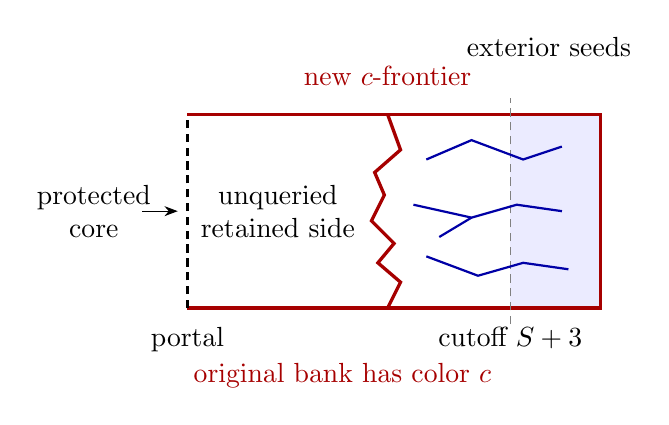
\begin{tikzpicture}[x=0.82cm,y=0.82cm,>=Stealth]
 \fill[blue!8] (6.6,0) rectangle (8,3);
 \draw[very thick,red!65!black] (1.6,0)--(8,0)--(8,3)--(1.6,3);
 \draw[densely dashed,thick] (1.6,0)--(1.6,3);
 \draw[densely dashed,gray] (6.6,-0.25)--(6.6,3.25);
 \draw[very thick,red!65!black]
 (4.7,0)--(4.9,0.4)--(4.55,0.7)--(4.8,1.0)--(4.45,1.35)
 --(4.65,1.75)--(4.5,2.1)--(4.9,2.45)--(4.7,3);
 \draw[thick,blue!65!black] (7.5,0.6)--(6.8,0.7)--(6.1,0.5)--(5.3,0.8);
 \draw[thick,blue!65!black] (7.4,1.5)--(6.7,1.6)--(6.0,1.4)--(5.1,1.6);
 \draw[thick,blue!65!black] (6.0,1.4)--(5.5,1.1);
 \draw[thick,blue!65!black] (7.4,2.5)--(6.8,2.3)--(6.0,2.6)--(5.3,2.3);
 \node[align=center] at (0.15,1.5) {protected\\core};
 \draw[->] (0.9,1.5)--(1.45,1.5);
 \node[below] at (1.6,-0.15) {portal};
 \node[align=center] at (3.0,1.5) {unqueried\\retained side};
 \node[above,red!65!black] at (4.7,3.3) {new \(c\)-frontier};
 \node[above] at (7.2,3.75) {exterior seeds};
 \node[below] at (6.6,-0.15) {cutoff \(S+3\)};
 \node[below,red!65!black] at (4.0,-0.7) {original bank has color \(c\)};
\end{tikzpicture}
\caption{Schematic shielding of one monochromatic cap.
The searched clusters, drawn in blue on the distal side, grow
from the exposed exterior region.
Their tested inner frontier is open in the bank color \(c\).
On success, all queried edges are on the frontier or to its
distal side; the retained region keeps an ordinary FK law.
The picture illustrates the separation argument and is not
an additional geometric assumption.}
\label{loc:fig-shield}
\end{figure}
\FloatBarrier

\Needspace{14\baselineskip}
\subsection{A uniform bound on the failure probability}
\begin{lemma}[The gate product estimate]
\label{loc:failure}
With the first \(J\) levels and their finite set \(H\) fixed,
let all \(H\)-cut preimages have diameter at most \(\rho\).
Uniformly conditional on the two explored heads, the probability
that the shielding procedure fails is bounded by
\begin{equation}
 \begin{aligned}
 &K|H|\rho^\alpha\\
 &\quad+K\sum_{k>J}2^k
     \prod_{j_*\le j<k}K\bigl(2^{-j}(j+2)^2\bigr)^\alpha\\
 &\quad+K\delta_n^{-2}
     \prod_{j_*\le j\le N_n}K\bigl(2^{-j}(j+2)^2\bigr)^\alpha
 +o(1).
 \end{aligned}
 \label{loc:failure-bound}
\end{equation}
Here \(j_*\) and the constants are independent of \(J,n\)
and of the unbounded part of the domain. In particular,
the failure probability tends to zero by first taking
\(J\) large, then \(\rho\) small at that stage, and finally
the mesh sufficiently small.
\end{lemma}

\begin{proof}
We compare all possible failure arms of one portal type
and one bank color together. Inside an annulus separated
from the portals and from the two ends of an arm, their
accessible side banks are free for the intruding color.
Lemma~\ref{geo:arm} applies to this union, including all
portal fragments and boundary-sector occurrences.
The comparison wires radial ends only; it counts actual
open arms and permits arbitrary off-shell conditioning.
It therefore gives product bounds in disjoint buffered
annuli without a factor for the number of fragments.
Earlier successful searches merely add favorable
single-color frontiers and do not change this argument.

If failure ends at a portal on an \(H\)-cut, the actual
intrusion arm from Lemma~\ref{loc:shield} joins a ball
containing that entire cut to a fixed outer radius,
say \(1/2\). The source is outside \(S+3-O(\delta_n)\),
whereas the cut lies inside \(S-2\). Applying
Lemma~\ref{geo:arm} to all fragments of that cut and
summing over the finitely many \(H\)-cuts gives the
first term in \eqref{loc:failure-bound}.

Now suppose failure ends at a circle-\(S\) portal.
Join its endpoint to \(0\) through the central core,
which excludes the initial \(H\)-caps and stays
inside radius \(S\), up to the fixed cell buffer.
Select a far point on the arm at radius \(S+2\).
This center-to-far-point route has the mandatory
initial gate sequence of Lemma~\ref{loc:gates}.

If any gate at a level \(j\le J\) is large, it lies
inside its selected parameter \(H\)-cap. The arm
therefore visits that cap, while its core extension
stays on the inner side. It crosses the corresponding
\(H\)-cut. This gives an arm through an annulus about
the physically tiny cut, again up to a bounded number
of cells. Circle-\(S\) portals are outside these
annuli because the \(H\)-cut lies inside \(S-2\).
The union comparison for the circle-portal type
therefore gives the same first term.

Otherwise let \(k>J\) be the first level at which
the gate is large. There are at most \(K2^k\)
choices for it, and each fixes all its ancestors.
The earlier ancestors are small.
Figure~\ref{loc:fig-gates} illustrates their surrounding annuli. For
\(j_*\le j<k\), the same arm crosses an annulus
with inner scale \(K2^{-j}\) and outer scale
\(c_0(j+2)^{-2}\). These annuli lie in disjoint
radial bands and miss the circle-\(S\) portals.
Both endpoints of the arm are outside the bands.
Applying the conditional product bound gives
\[
 K2^k\prod_{j_*\le j<k}
       K\bigl(2^{-j}(j+2)^2\bigr)^\alpha .
 \]
The two possible bank colors cost only another
fixed factor.

Finally, if all gates through \(N_n\) are small,
specify the connected initial-domain sector of an incident
cell at the first crossing of radius \(S+2\).
That sector fixes the ancestor chain, since it is connected
and lies outside all the tested circles. The angle bound
gives cell areas at least \(c_\eta\delta_n^2\)
and bounded local degree. A bounded annular band
therefore has at most \(K\delta_n^{-2}\)
possible terminal cells and sectors. The product
through \(N_n\) gives the last term.

For completeness, the logarithm of the product
through \(k\) is
\[
 -\frac{\alpha\log2}{2}k^2+O(k\log(k+2)).
 \]
It dominates both the factor \(2^k\) and,
when \(k=N_n\), the factor
\(\delta_n^{-2}=\exp(O(N_n))\).
The last term vanishes, and the tail sum can be
made arbitrarily small by increasing \(J\).
At every fixed stage the number \(|H|\) is finite,
so \(\rho\) can then make the first term small.
Cell buffers and generic contour perturbations
are absorbed once the stage is fixed and the
mesh is sufficiently small. All comparison
annuli have uniformly bounded physical radii.
\end{proof}

\begin{figure}[tb]
\centering
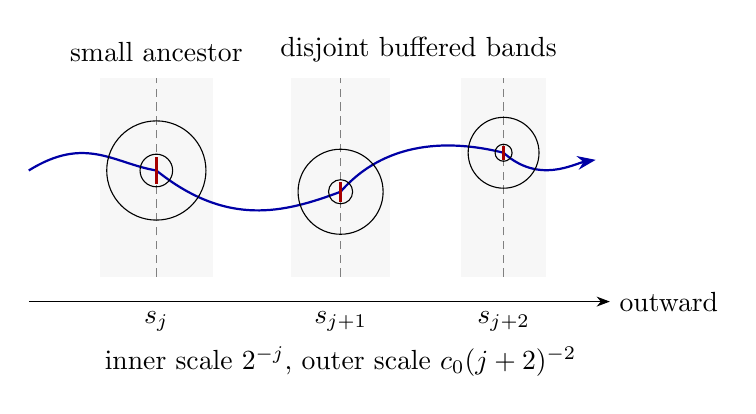
\begin{tikzpicture}[x=0.9cm,y=0.9cm,>=Stealth]
 \fill[gray!6] (1.0,-1.4) rectangle (2.6,1.4);
 \fill[gray!6] (3.7,-1.4) rectangle (5.1,1.4);
 \fill[gray!6] (6.1,-1.4) rectangle (7.3,1.4);
 \draw[->] (0,-1.75)--(8.2,-1.75) node[right] {outward};
 \foreach \x/\lab in {1.8/{s_j},4.4/{s_{j+1}},6.7/{s_{j+2}}}
 {
   \draw[densely dashed,gray] (\x,-1.4)--(\x,1.4);
   \node[below] at (\x,-1.75) {\(\lab\)};
 }
 \draw[blue!65!black,thick,->]
 (0,0.1)..controls(0.8,0.6)and(1.2,0.2)..(1.8,0.1)
 ..controls(2.8,-0.7)and(3.6,-0.5)..(4.4,-0.2)
 ..controls(5.1,0.6)and(6.1,0.5)..(6.7,0.35)
 ..controls(7.2,-0.1)and(7.7,0.2)..(8,0.25);
 \draw[red!65!black,very thick] (1.8,-0.09)--(1.8,0.29);
 \draw[red!65!black,very thick] (4.4,-0.34)--(4.4,-0.06);
 \draw[red!65!black,very thick] (6.7,0.25)--(6.7,0.45);
 \draw (1.8,0.1) circle (0.7);
 \draw (1.8,0.1) circle (0.23);
 \draw (4.4,-0.2) circle (0.6);
 \draw (4.4,-0.2) circle (0.17);
 \draw (6.7,0.35) circle (0.5);
 \draw (6.7,0.35) circle (0.12);
 \node[above] at (1.8,1.5) {small ancestor};
 \node[above] at (5.5,1.5) {disjoint buffered bands};
 \node[align=center] at (4.4,-2.6)
 {inner scale \(2^{-j}\), outer scale \(c_0(j+2)^{-2}\)};
\end{tikzpicture}
\caption{Schematic gate hierarchy, with the radial direction
flattened for clarity. Short segments mark gates, pairs of circles
bound their annuli, and shaded strips mark disjoint radial bands.
The curved intrusion arm visits each mandatory
small ancestor and therefore crosses every surrounding annulus.
The exponentially small inner scales and polynomially spaced
outer scales give the product in \eqref{loc:failure-bound}.}
\label{loc:fig-gates}
\end{figure}
\FloatBarrier

\subsection{Reduction, mixtures, and the full theorem}

\begin{proposition}[Reduction to bounded Dobrushin problems]
\label{loc:reduction}
From every admissible approximation sequence one can extract
a further subsequence and perform finite edge revelations
with success probability tending to one, so that on success:
\begin{enumerate}
\item the unqueried connecting domain \(\widehat\Omega_n\)
is a Dobrushin polygon on the original mesh with the
same thermal parameters and diameter at most \(2S+20\);
\item conditional on the complete revelation record, its
interface has the ordinary Dobrushin FK law;
\item every deterministic sequence of possible successful
outputs \((\widehat\Omega_n,\widehat a_n,\widehat b_n)\)
converges in the marked Carath\'eodory sense to
\((\Omega,a,b)\);
\item the normalized coordinates on the retained domain
are uniformly \(o(1)\) from its original normalized
coordinates, including prime-end occurrences, and
the removed endpoint heads have vanishing disc
diameter.
\end{enumerate}
All error bounds are uniform over successful outcomes.
\end{proposition}

\begin{proof}
Let the prescribed parameter accuracy and failure
probability decrease to zero in stages. At one stage,
choose \(J\) so that the tail in
\eqref{loc:failure-bound} is smaller than its failure
tolerance. Pass to the subsequence determining the
finite set \(H\). Choose endpoint fences with the
prescribed small parameter size and protect their
access chains. Next choose the \(H\)-caps with
still smaller parameter size and physical cut
diameter \(\rho\) making the first term of
\eqref{loc:failure-bound} small. Only then take
the mesh small enough for all deterministic
contour and cell comparisons at that stage.
Iterate and take a diagonal subsequence.

On success, Lemma~\ref{loc:shield} has removed
all parts beyond \(S+3+K\delta_n\).
The central core and the two front corners
remain, and every new boundary is a wired
extension of one original bank. This proves
the uniform diameter assertion and the
conditional-law assertion. The failure
probability tends to zero by
Lemma~\ref{loc:failure}.

It remains to verify coordinate control
uniformly in the explored outcomes.
In initial disc coordinates, the removed
heads and their filled components are
small attached obstructions by
Lemma~\ref{loc:heads}. Thus their removal
changes normalized coordinates by \(o(1)\)
along the diagonal stages, by
Lemma~\ref{loc:obstructions}.

The portals in the resulting domain also
have uniformly vanishing parameter
diameter. For the \(H\)-portals this follows
from their chosen angular sizes. For
circle-\(S\) portals it follows from
Lemma~\ref{loc:remote}, since the entire
circle is outside \(B(0,S-1)\).
Their noncentral shadows are consequently
small. Every subsequent searched or
discarded portion lies behind one of
these portals. Its points attach to the
old boundary within that small shadow.
Any remaining boundary-cell modifications
have vanishing parameter diameter by
Lemma~\ref{geo:crosscut} and attach
through their incident sectors.
Filling discarded components preserves
the small attachment property.
A second application of
Lemma~\ref{loc:obstructions} therefore
gives uniform \(o(1)\) closeness between
the final and initial normalized maps.

In particular all fixed kernel compacts
are eventually unmodified; the successive
cuts lie in parameter neighborhoods
shrinking to the circle. The two new
marks are within the endpoint fence
neighborhoods, whose diameters tend to
zero. This proves marked Carath\'eodory
convergence of every deterministic
sequence of successful outputs. The
same reasoning is uniform over outcomes,
because only the deterministic stage
tolerances, cell sizes, and parameter
shadows were used.

Finally the original curve on success
is the first head, followed by the
retained interface, followed by the
reverse of the second head. Its
middle part is exactly the ordinary
conditional interface already described.
Uniform coordinate closeness and
vanishing head diameters show that
this concatenation and the retained
curve have distance \(o(1)\) in the
oriented uniform metric modulo
increasing reparametrization. One may
allocate a vanishing parameter interval
to each head, or use continuous
nondecreasing reparametrizations and
approximate them by strictly increasing
ones. This proves the last assertion.
\end{proof}

\begin{corollary}[Universality without a diameter assumption]
\label{loc:universality}
For \(m>0\), every approximation sequence in
Theorem~\ref{thm:main} converges to the law of
Definition~\ref{def:law}, in the specified
normalized-disc curve topology.
\end{corollary}

\begin{proof}
Apply Proposition~\ref{loc:reduction} to any subsequence.
Conditional on a successful record, the retained law
is one of the bounded laws of
Proposition~\ref{uni:bounded}. Their convergence is
uniform over the possible successful outputs in
the required sequential sense. Indeed, if a
bounded continuous test function of curves
had an error bounded below along some sequence
of outputs, choosing one such output at
each mesh would contradict that proposition,
since every chosen domain sequence has
the same marked limit and a common diameter
bound.

Integrate this convergence against the
distribution of the successful records.
The failure probability vanishes, and
the original and retained curves have
vanishing distance on success.
Thus this further subsequence converges
to the same continuum law. Every
subsequence admits such a further
subsequence, which proves full-sequence
convergence. In particular the limiting
law is independent of the lattices,
domain approximations, and nome sequence.
\end{proof}

\paragraph{Negative mass and completion of the theorem.}
For \(m<0\), exchange primal and dual vertices and
the corresponding rhombus diagonals. The prescribed
negative abstract angle is the complement of the
positive abstract angle at the complementary
geometric half-angle. Hence the two sine factors
in the loop weight are exchanged exactly, while
the number of closed loops and the angle bound
are preserved. The two boundary banks exchange
roles. Apply the positive-mass construction on
the dual domain with the starting and terminal
marks interchanged, and reverse the resulting
oriented path. Any boundary half-cell adjustment
has vanishing normalized diameter by
Lemma~\ref{geo:crosscut} and the attachment
argument above. This yields the claimed
continuum characterization and full-sequence
universality for the negative branch as well.
Together with Proposition~\ref{uni:bounded},
Corollary~\ref{loc:universality} proves
Theorem~\ref{thm:main}.

\phantomsection
\addcontentsline{toc}{section}{References}
\begin{thebibliography}{99}

\bibitem{CDCHKS}
Dmitry Chelkak, Hugo Duminil-Copin, Cl\'ement Hongler,
Antti Kemppainen, and Stanislav Smirnov,
\emph{Convergence of Ising interfaces to Schramm's SLE curves},
Comptes Rendus. Math\'ematique \textbf{352} (2014), no.~2, 157--161.
\href{https://doi.org/10.1016/j.crma.2013.12.002}{doi:10.1016/j.crma.2013.12.002}.
\href{https://arxiv.org/abs/1312.0533v2}{arXiv:1312.0533v2}.

\bibitem{CS}
Dmitry Chelkak and Stanislav Smirnov,
\emph{Universality in the 2D Ising model and conformal invariance of fermionic observables},
Inventiones Mathematicae \textbf{189} (2012), no.~3, 515--580.
\href{https://doi.org/10.1007/s00222-011-0371-2}{doi:10.1007/s00222-011-0371-2}.
\href{https://arxiv.org/abs/0910.2045v2}{arXiv:0910.2045v2}.

\bibitem{KS}
Antti Kemppainen and Stanislav Smirnov,
\emph{Random curves, scaling limits and Loewner evolutions},
Annals of Probability \textbf{45} (2017), no.~2, 698--779.
\href{https://doi.org/10.1214/15-AOP1074}{doi:10.1214/15-AOP1074}.
The version used for numbered statements is
\href{https://arxiv.org/abs/1212.6215v3}{arXiv:1212.6215v3} (2015).

\bibitem{Lawler}
Gregory~F. Lawler,
\emph{Stochastic Calculus: An Introduction with Applications},
author-hosted text, revised 15 February 2023.
\url{https://www.math.uchicago.edu/~lawler/finbook.pdf}.

\bibitem{MS}
Nikolai Makarov and Stanislav Smirnov,
\emph{Off-critical lattice models and massive SLEs},
in \emph{XVIth International Congress on Mathematical Physics},
World Scientific, Hackensack, NJ, 2010, pp.~362--371.
\href{https://doi.org/10.1142/9789814304634_0024}{doi:10.1142/9789814304634\_0024}.
\href{https://arxiv.org/abs/0909.5377v1}{arXiv:0909.5377v1} (2009).

\bibitem{Park}
S.~C. Park,
\emph{Convergence of fermionic observables in the massive planar FK-Ising model},
Communications in Mathematical Physics \textbf{396} (2022), 1071--1133.
\href{https://doi.org/10.1007/s00220-022-04488-6}{doi:10.1007/s00220-022-04488-6}.
The version used for numbered statements is
\href{https://arxiv.org/abs/2103.04649v3}{arXiv:2103.04649v3} (2022).

\bibitem{Pommerenke}
Christian Pommerenke,
\emph{Boundary Behaviour of Conformal Maps},
Grundlehren der mathematischen Wissenschaften, vol.~299,
Springer-Verlag, Berlin, 1992.
\href{https://doi.org/10.1007/978-3-662-02770-7}{doi:10.1007/978-3-662-02770-7}.

\bibitem{Smirnov}
Stanislav Smirnov,
\emph{Conformal invariance in random cluster models.
I. Holomorphic fermions in the Ising model},
Annals of Mathematics \textbf{172} (2010), no.~2, 1435--1467.
\href{https://doi.org/10.4007/annals.2010.172.1435}{doi:10.4007/annals.2010.172.1435}.
\href{https://arxiv.org/abs/0708.0039}{arXiv:0708.0039}.

\end{thebibliography}

\end{document}
